%%
%% Template appendix.tex
%%

\appendix

\chapter{How to Obtain the Datasets}
\label{cha:datasets}

The following SQL query is used to get the main SDSS dataset containing 2.8 million
labelled objects from the Sloan SkyServer:\footnote{
	\url{http://skyserver.sdss.org/CasJobs/}}

\begin{minted}[fontsize=\footnotesize, frame=single, tabsize=4]{sql}
SELECT
	-- right ascension and declination in degrees
	p.ra, p.dec,
	
	-- class of object, expert opinion (galaxy, star, or quasar)
	CASE s.class WHEN 'GALAXY' THEN 'Galaxy'
				 WHEN 'STAR' THEN 'Star'
				 WHEN 'QSO' THEN 'Quasar'
				 END AS class,
	
	s.subclass, -- subclass of object
	
	-- redshift of object from spectrum with error, expert opinion
	s.z AS redshift,
	s.zErr AS redshiftErr,
	s.zWarning,
	
	-- PSF and Petrosian mags in 5 bands (ugriz) with error
	p.psfMag_u, p.psfMagErr_u,
	p.psfMag_g, p.psfMagErr_g,
	p.psfMag_r, p.psfMagErr_r,
	p.psfMag_i, p.psfMagErr_i,
	p.psfMag_z, p.psfMagErr_z,
	
	p.petroMag_u, p.petroMagErr_u,
	p.petroMag_g, p.petroMagErr_g,
	p.petroMag_r, p.petroMagErr_r,
	p.petroMag_i, p.petroMagErr_i,
	p.petroMag_z, p.petroMagErr_z,
	
	-- extinction values
	p.extinction_u, p.extinction_g, p.extinction_r,
	p.extinction_i, p.extinction_z,
	
	-- size measurement in r-band in arc seconds
	p.petroRad_r, p.petroRadErr_r

FROM PhotoObj AS p
JOIN SpecObj AS s
ON s.bestobjid = p.objid

WHERE
	-- only include objects with complete and reasonably accurate data
	p.psfMagErr_u BETWEEN 0 AND 3
	AND p.psfMagErr_g BETWEEN 0 AND 3
	AND p.psfMagErr_r BETWEEN 0 AND 3
	AND p.psfMagErr_i BETWEEN 0 AND 3
	AND p.psfMagErr_z BETWEEN 0 AND 3
	AND p.petroMagErr_u BETWEEN 0 AND 3
	AND p.petroMagErr_g BETWEEN 0 AND 3
	AND p.petroMagErr_r BETWEEN 0 AND 3
	AND p.petroMagErr_i BETWEEN 0 AND 3
	AND p.petroMagErr_z BETWEEN 0 AND 3
	AND p.petroRadErr_r BETWEEN 0 AND 3
	AND s.zErr BETWEEN 0 AND 0.1
	AND s.zWarning = 0    -- spectrum is ok
\end{minted}


The following query is used to extract photometric measurements from all 800 million
in the database. Since the file is fairly big (around 200 GB in size),
a special request might need to be made.

\begin{minted}[fontsize=\footnotesize, frame=single, tabsize=4]{sql}
SELECT
	p.ra, p.dec,
	CASE s.class WHEN 'GALAXY' THEN 'Galaxy'
				 WHEN 'STAR' THEN 'Star'
				 WHEN 'QSO' THEN 'Quasar'
				 END AS class,
	s.subclass,
	s.z AS redshift,
	s.zErr AS redshiftErr,
	s.zWarning,
	p.psfMag_u, p.psfMagErr_u,
	p.psfMag_g, p.psfMagErr_g,
	p.psfMag_r, p.psfMagErr_r,
	p.psfMag_i, p.psfMagErr_i,
	p.psfMag_z, p.psfMagErr_z,
	p.petroMag_u, p.petroMagErr_u,
	p.petroMag_g, p.petroMagErr_g,
	p.petroMag_r, p.petroMagErr_r,
	p.petroMag_i, p.petroMagErr_i,
	p.petroMag_z, p.petroMagErr_z,
	p.extinction_u, p.extinction_g, p.extinction_r,
	p.extinction_i, p.extinction_z,
	p.petroRad_r, p.petroRadErr_r
FROM PhotoObj AS p
LEFT JOIN SpecObj AS s
ON s.bestobjid = p.objid
\end{minted}






%\chapter{Guide to Using mclearn}
%\label{cha:mclearn}

%\section{Installation}
%\label{sub:installation}

%\section{Usage and Examples}
%\label{sub:usage}


%\chapter{Vectorisation of the Variance Estimation}
%\label{cha:vectorise}

%In estimating the variance of the unlabelled pool, there are two matrices we wish to compute...



\chapter{Dust Extinction Vectors} \index{dust extinction}
\label{cha:dustvectors}

The SDF98 extinction values are given in the SDSS dataset. To calculate the other
two extinction vectors, we start with a reference reddening quantity
\begin{IEEEeqnarray*}{lCl}
	E_{B-V} &=& \frac{\A_r}{2.751}
\end{IEEEeqnarray*}
where $\A_r$ is the SDF98 extinction value in the r-band.

As a check, we can actually recover the SDF98 extinction vector as follows:
\begin{IEEEeqnarray*}{lCl}
	\A_u &=& 5.155 \cdot E_{B-V} \\
	\A_g &=& 3.793 \cdot E_{B-V} \\
	\A_r &=& 2.751 \cdot E_{B-V} \\
	\A_i &=& 2.086 \cdot E_{B-V} \\
	\A_z &=& 1.479 \cdot E_{B-V}
\end{IEEEeqnarray*}
Later, \citeN{schlafly11} applied a different extinction curve, giving us the following
correction values:
\begin{IEEEeqnarray*}{lCl}
	\A_u &=& 4.239 \cdot E_{B-V} \\
	\A_g &=& 3.303 \cdot E_{B-V} \\
	\A_r &=& 2.285 \cdot E_{B-V} \\
	\A_i &=& 1.698 \cdot E_{B-V} \\
	\A_z &=& 1.263 \cdot E_{B-V}
\end{IEEEeqnarray*}
Recently, \citeN{wolf14} remapped the $E_{B-V}$ scale to
\begin{IEEEeqnarray*}{lCl}
	E'_{B-V} &=&
	\begin{cases}
		E_{B-V} & \text{if } E_{B-V} \in [0, 0.04], \\
		E_{B-V} + 0.5(E_{B-V} - 0.04) & \text{if } E_{B-V} \in [0, 0.08], \\
		E_{B-V} + 0.02 & \text{if } E_{B-V} \in [0.08, +\infty].
	\end{cases}
\end{IEEEeqnarray*}
which can then be used to calculate a new set of correction values:
\begin{IEEEeqnarray*}{lCl}
	\A_u &=& 4.305 \cdot E'_{B-V} \\
	\A_g &=& 3.288 \cdot E'_{B-V} \\
	\A_r &=& 2.261 \cdot E'_{B-V} \\
	\A_i &=& 1.714 \cdot E'_{B-V} \\
	\A_z &=& 1.263 \cdot E'_{B-V}
\end{IEEEeqnarray*}
Each of these correction values need to be subtracted from the corresponding magnitudes
to make up for the loss of the scattered light.





\chapter{Supplementary Results}
\label{cha:supp}

In this Appendix, we present results that are not vital to the main narrative but still somewhat
interesting.

%\section{Reliability of Probabilities Estimates}
%\label{sec:forest_prob}
%
%Figure \ref{fig:forest_multinom} shows the learning curves
%
%We found that the probabilities estimated by both random forests and multinomial regression
%to be unreliable. [To do: include learning curves of random forest, one-vs-rest, and
%multinomial regression, and warm-start here, test both SDSS and VST ATLAS]
%
%\begin{figure}[p]
%	\centering
%	\begin{subfigure}{\textwidth}
%		\centering
%		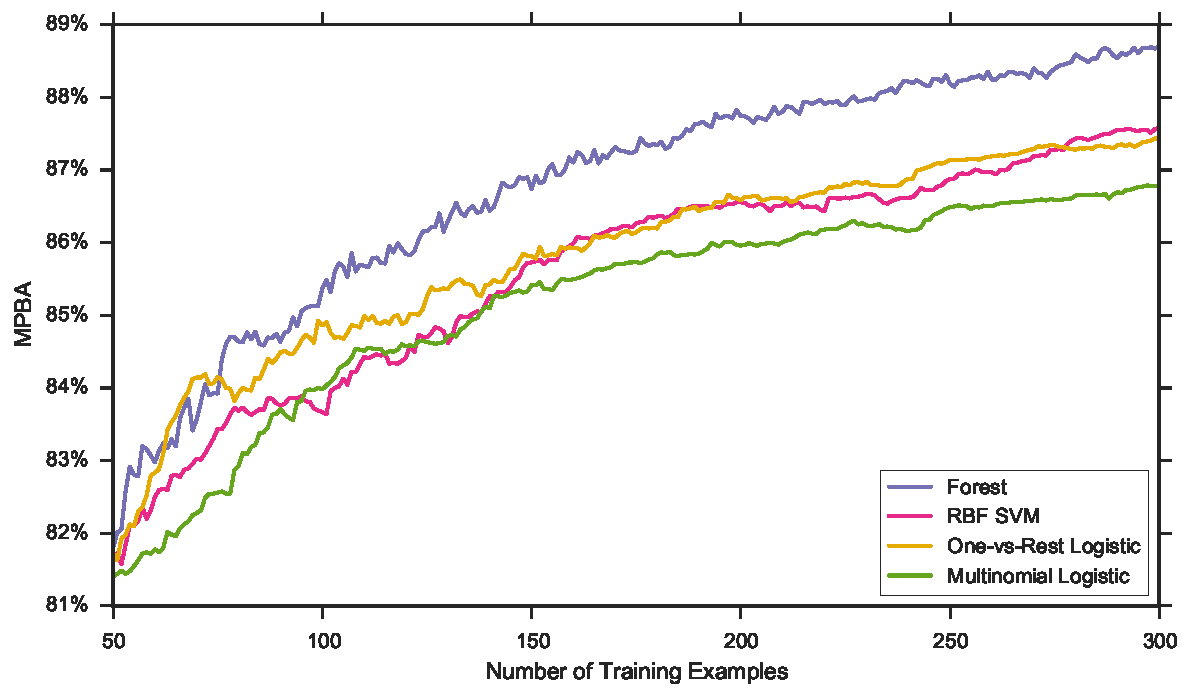
\includegraphics[width=\textwidth]{figures/appendix/sdss_forest_multinom}
%		\caption{SDSS dataset}
%		\label{fig:sdss_forest_multinom}
%	\end{subfigure}\\
%	\begin{subfigure}{\textwidth}
%		\centering
%		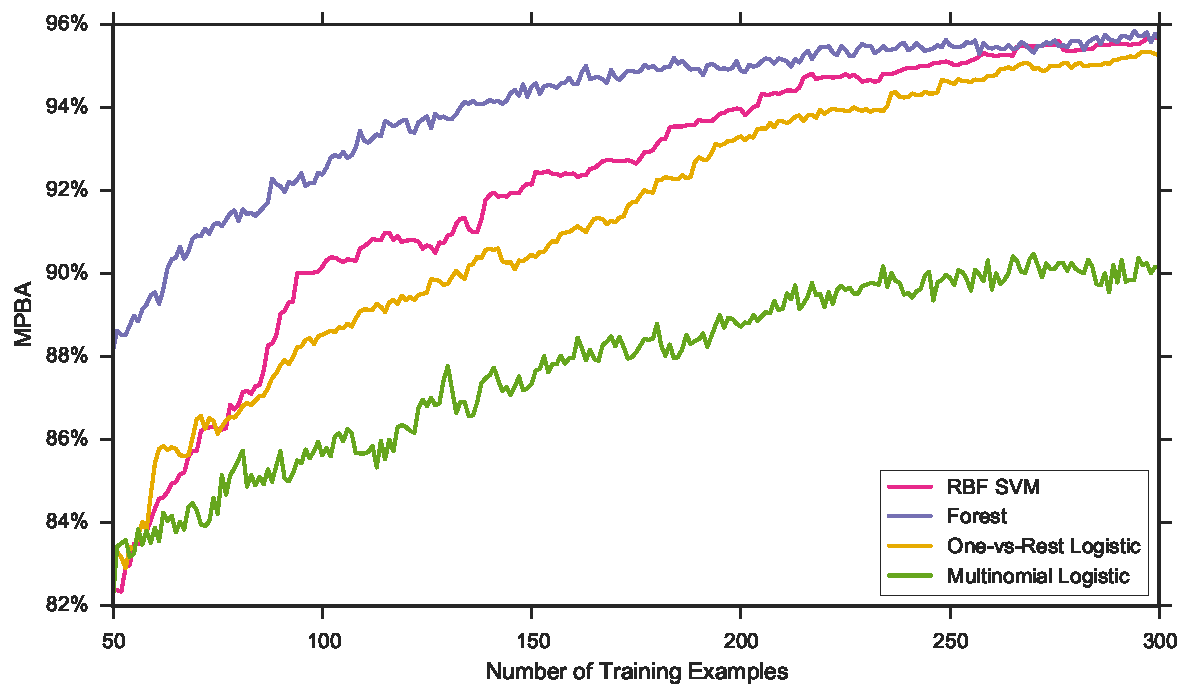
\includegraphics[width=\linewidth]{figures/appendix/vstatlas_forest_multinom}
%		\caption{VST ATLAS dataset}
%		\label{fig:vstatlas_forest_multinom}
%	\end{subfigure}
%	\caption[Reliability of probability estimates]{Learning curves of various classifiers: }
%	\label{fig:forest_multinom}
%\end{figure}


\section{Effects of Dust Extinction on Recall}

In Chapter \ref{cha:expt1} we tested the effects of three different extinction vectors 
on the accuracy rate. Figure \ref{fig:map_recall_uncorrected} shows how the recall rate is distributed
over the celestial sphere. Overall, the recall on galaxies is almost perfect, while
the recall on stars is fairly average. On the three pages after that, Figures \ref{fig:map_recall_sfd98}, \ref{fig:map_recall_sf11}, and \ref{fig:map_recall_w14} show
the improvement on recall after each extinction vector is applied. The interesting bit
is that there is a patch of stars right next to the Milky Way plane that gets a big improvement
in recall after reddening correction. Thus the extinction vector would be very important
if there were more objects that are closer to the Milky Way plane (which is the case in the SkyMapper project).


\begin{figure}[p]
	\centering
	\begin{subfigure}{\textwidth}
		\centering
		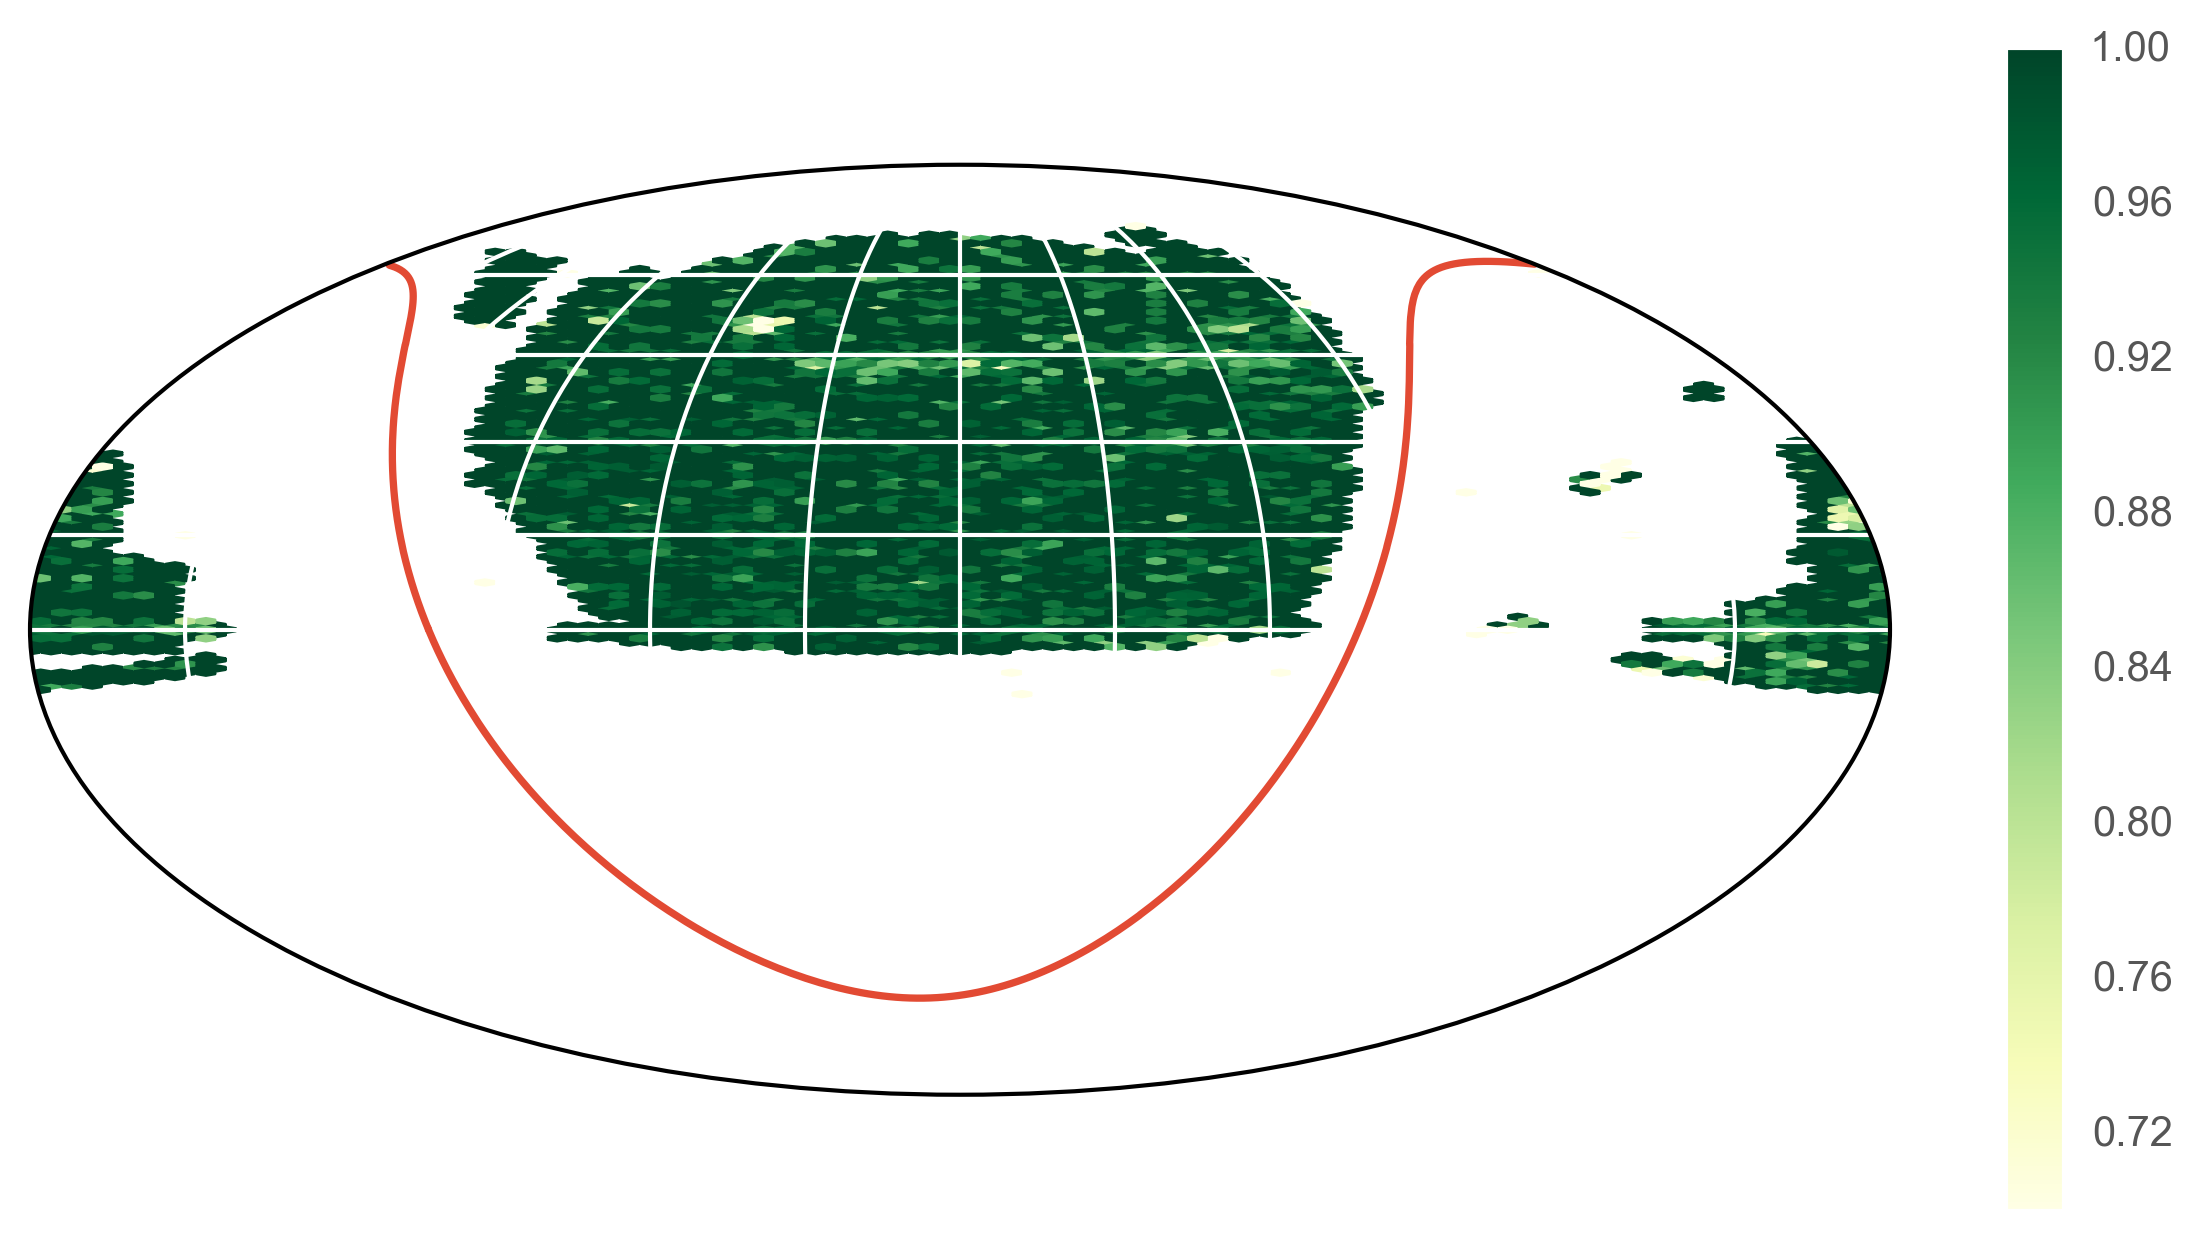
\includegraphics[width=0.75\textwidth]{figures/appendix/map_recall_uncorrected_Galaxy}
		\caption{Recall map of galaxies.}
		\label{fig:map_recall_uncorrected_galaxies}
	\end{subfigure}\\
	\begin{subfigure}{\textwidth}
		\centering
		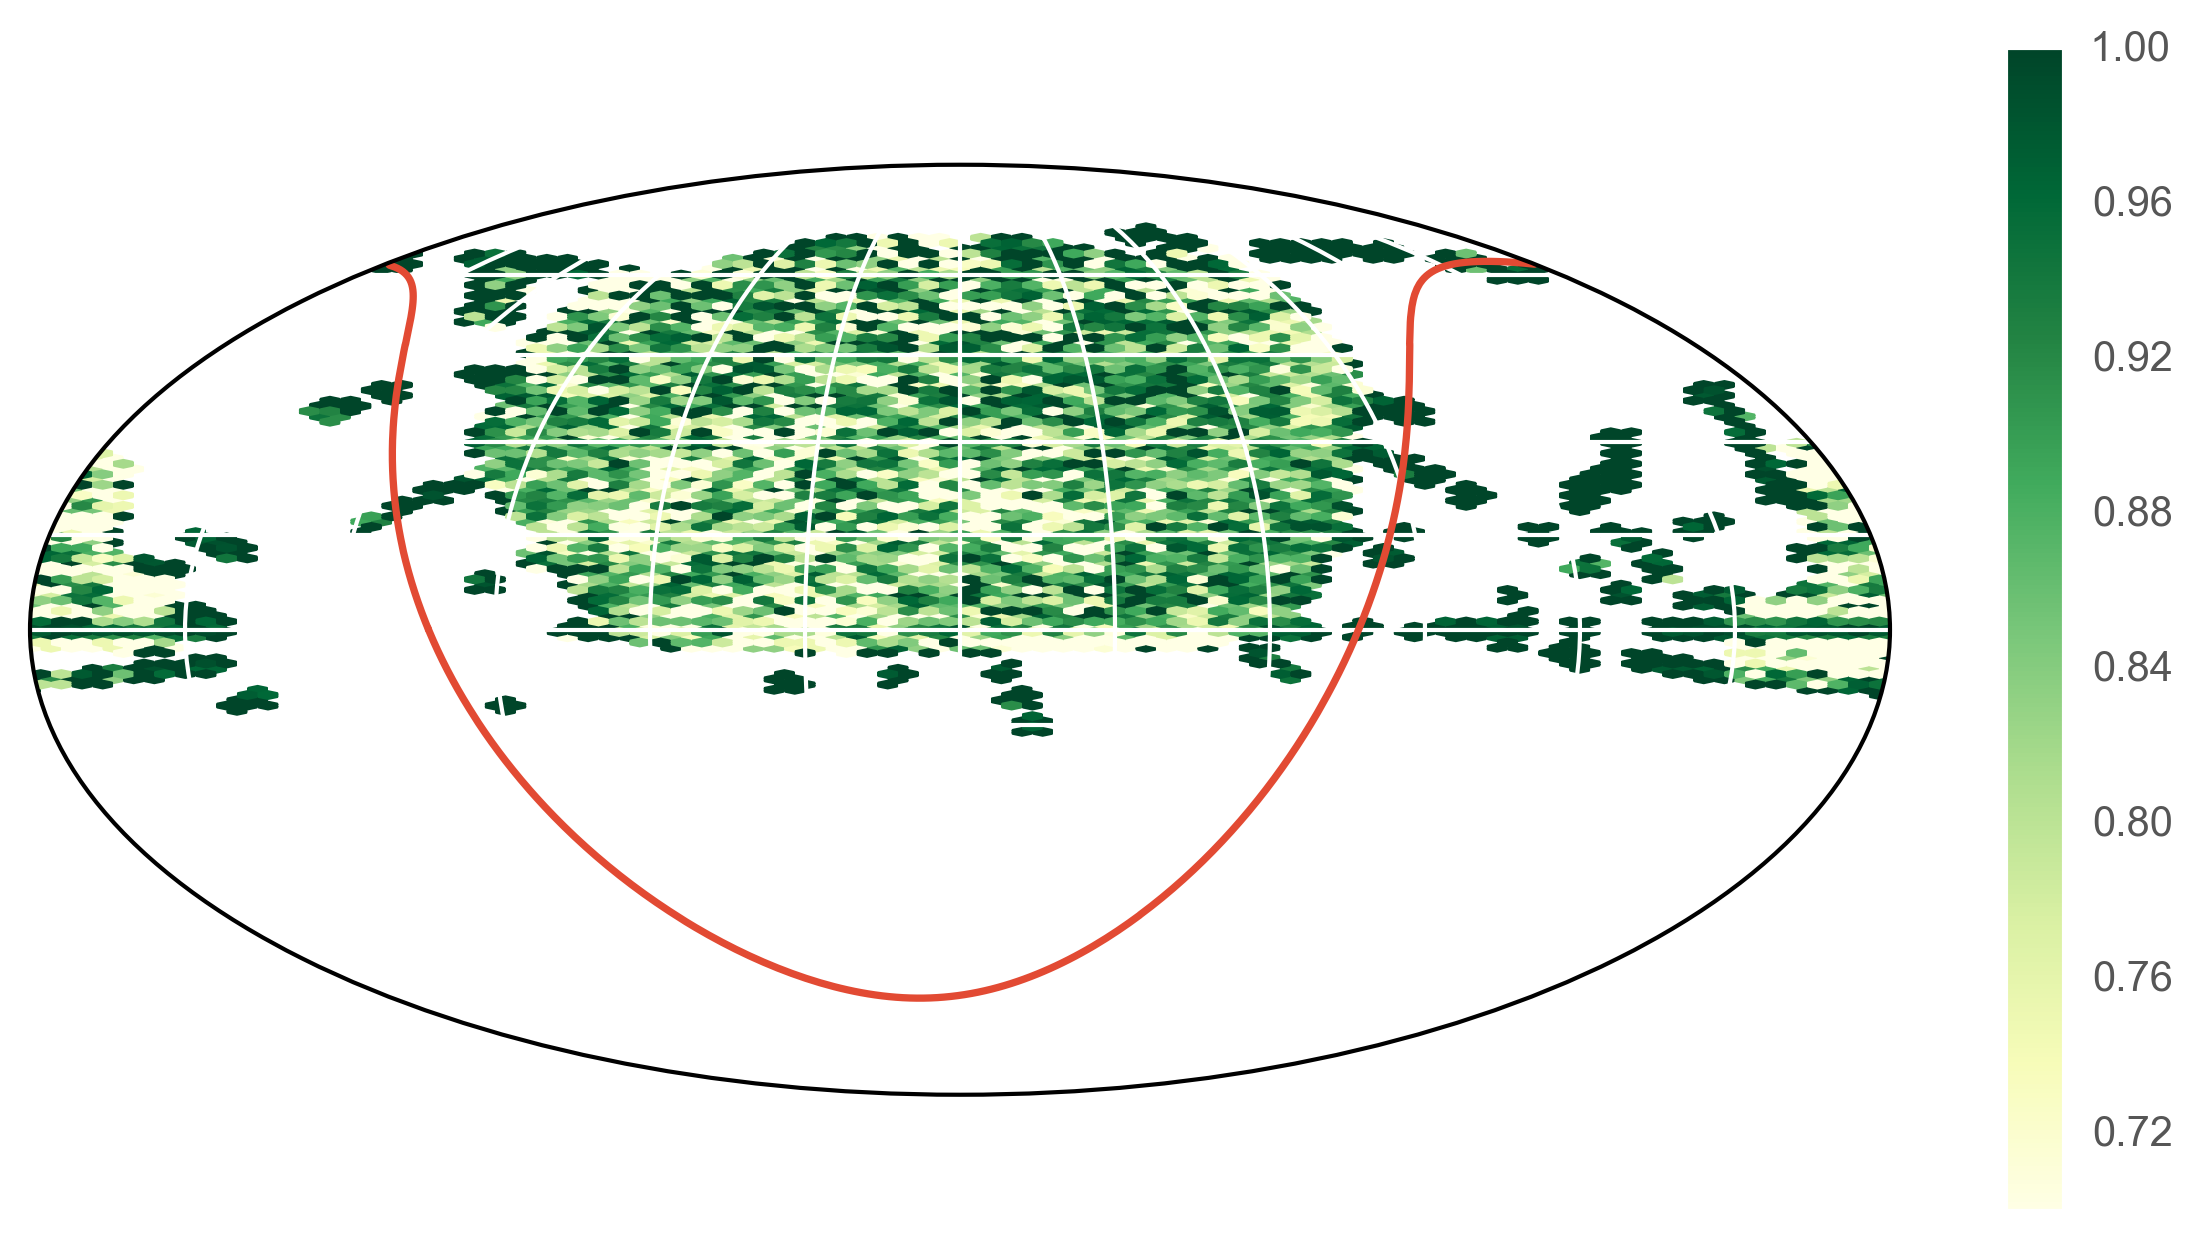
\includegraphics[width=0.75\linewidth]{figures/appendix/map_recall_uncorrected_Star}
		\caption{Recall map of stars.}
		\label{fig:map_recall_uncorrected_stars}
	\end{subfigure}
	\begin{subfigure}{\textwidth}
		\centering
		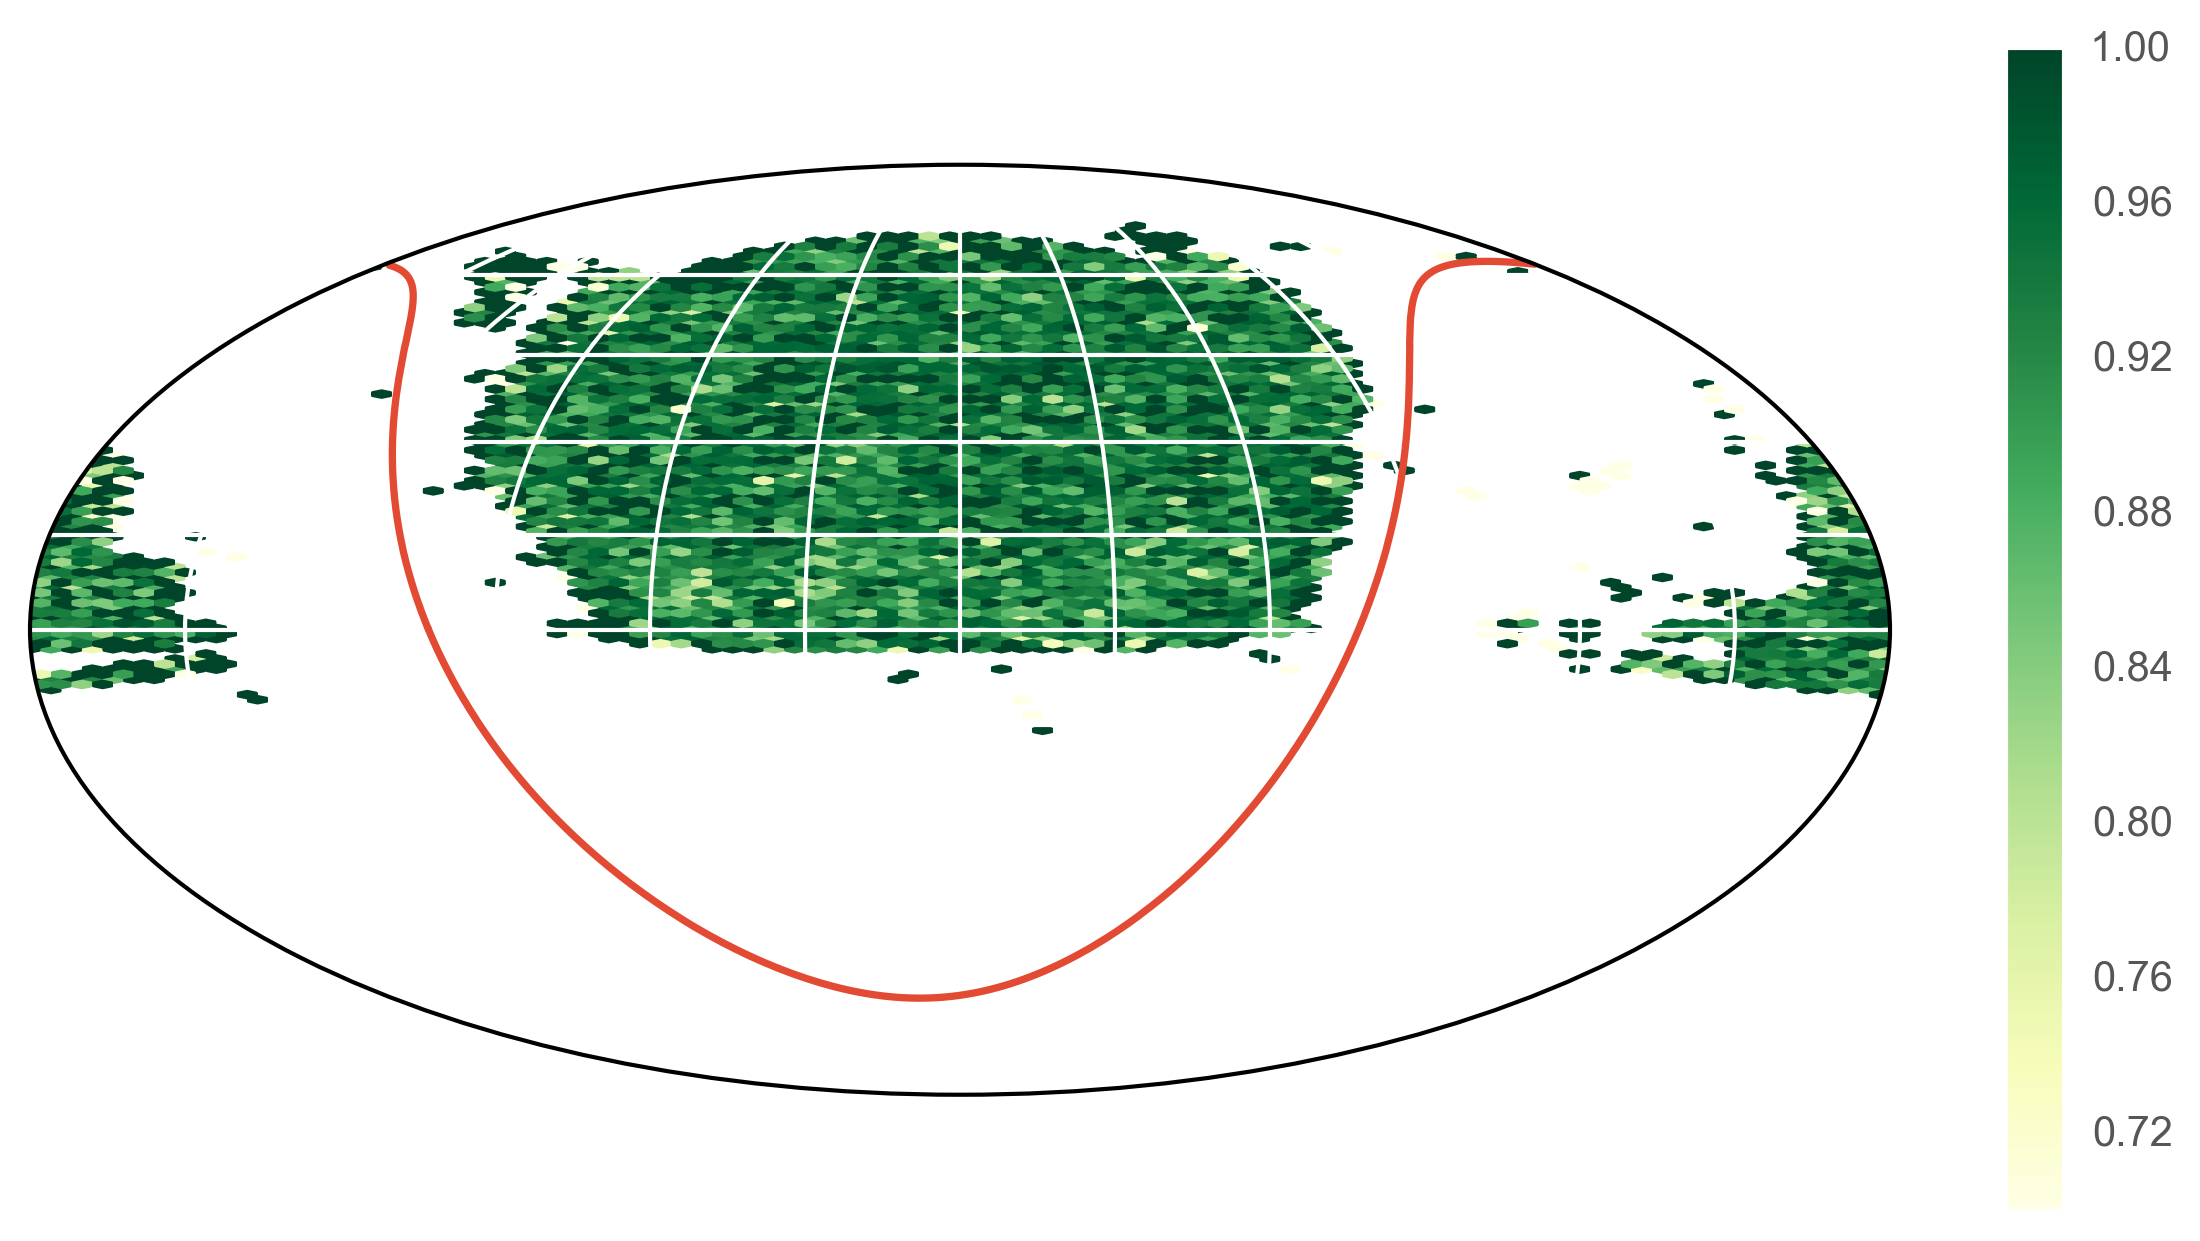
\includegraphics[width=0.75\linewidth]{figures/appendix/map_recall_uncorrected_Quasar}
		\caption{Recall map of quasars.}
		\label{fig:map_recall_uncorrected_quasars}
	\end{subfigure}
	\caption[Recall maps when there is no corrections]{
        Recall maps when there is no corrections.}
	\label{fig:map_recall_uncorrected}
\end{figure}


\begin{figure}[p]
	\centering
	\begin{subfigure}{\textwidth}
		\centering
		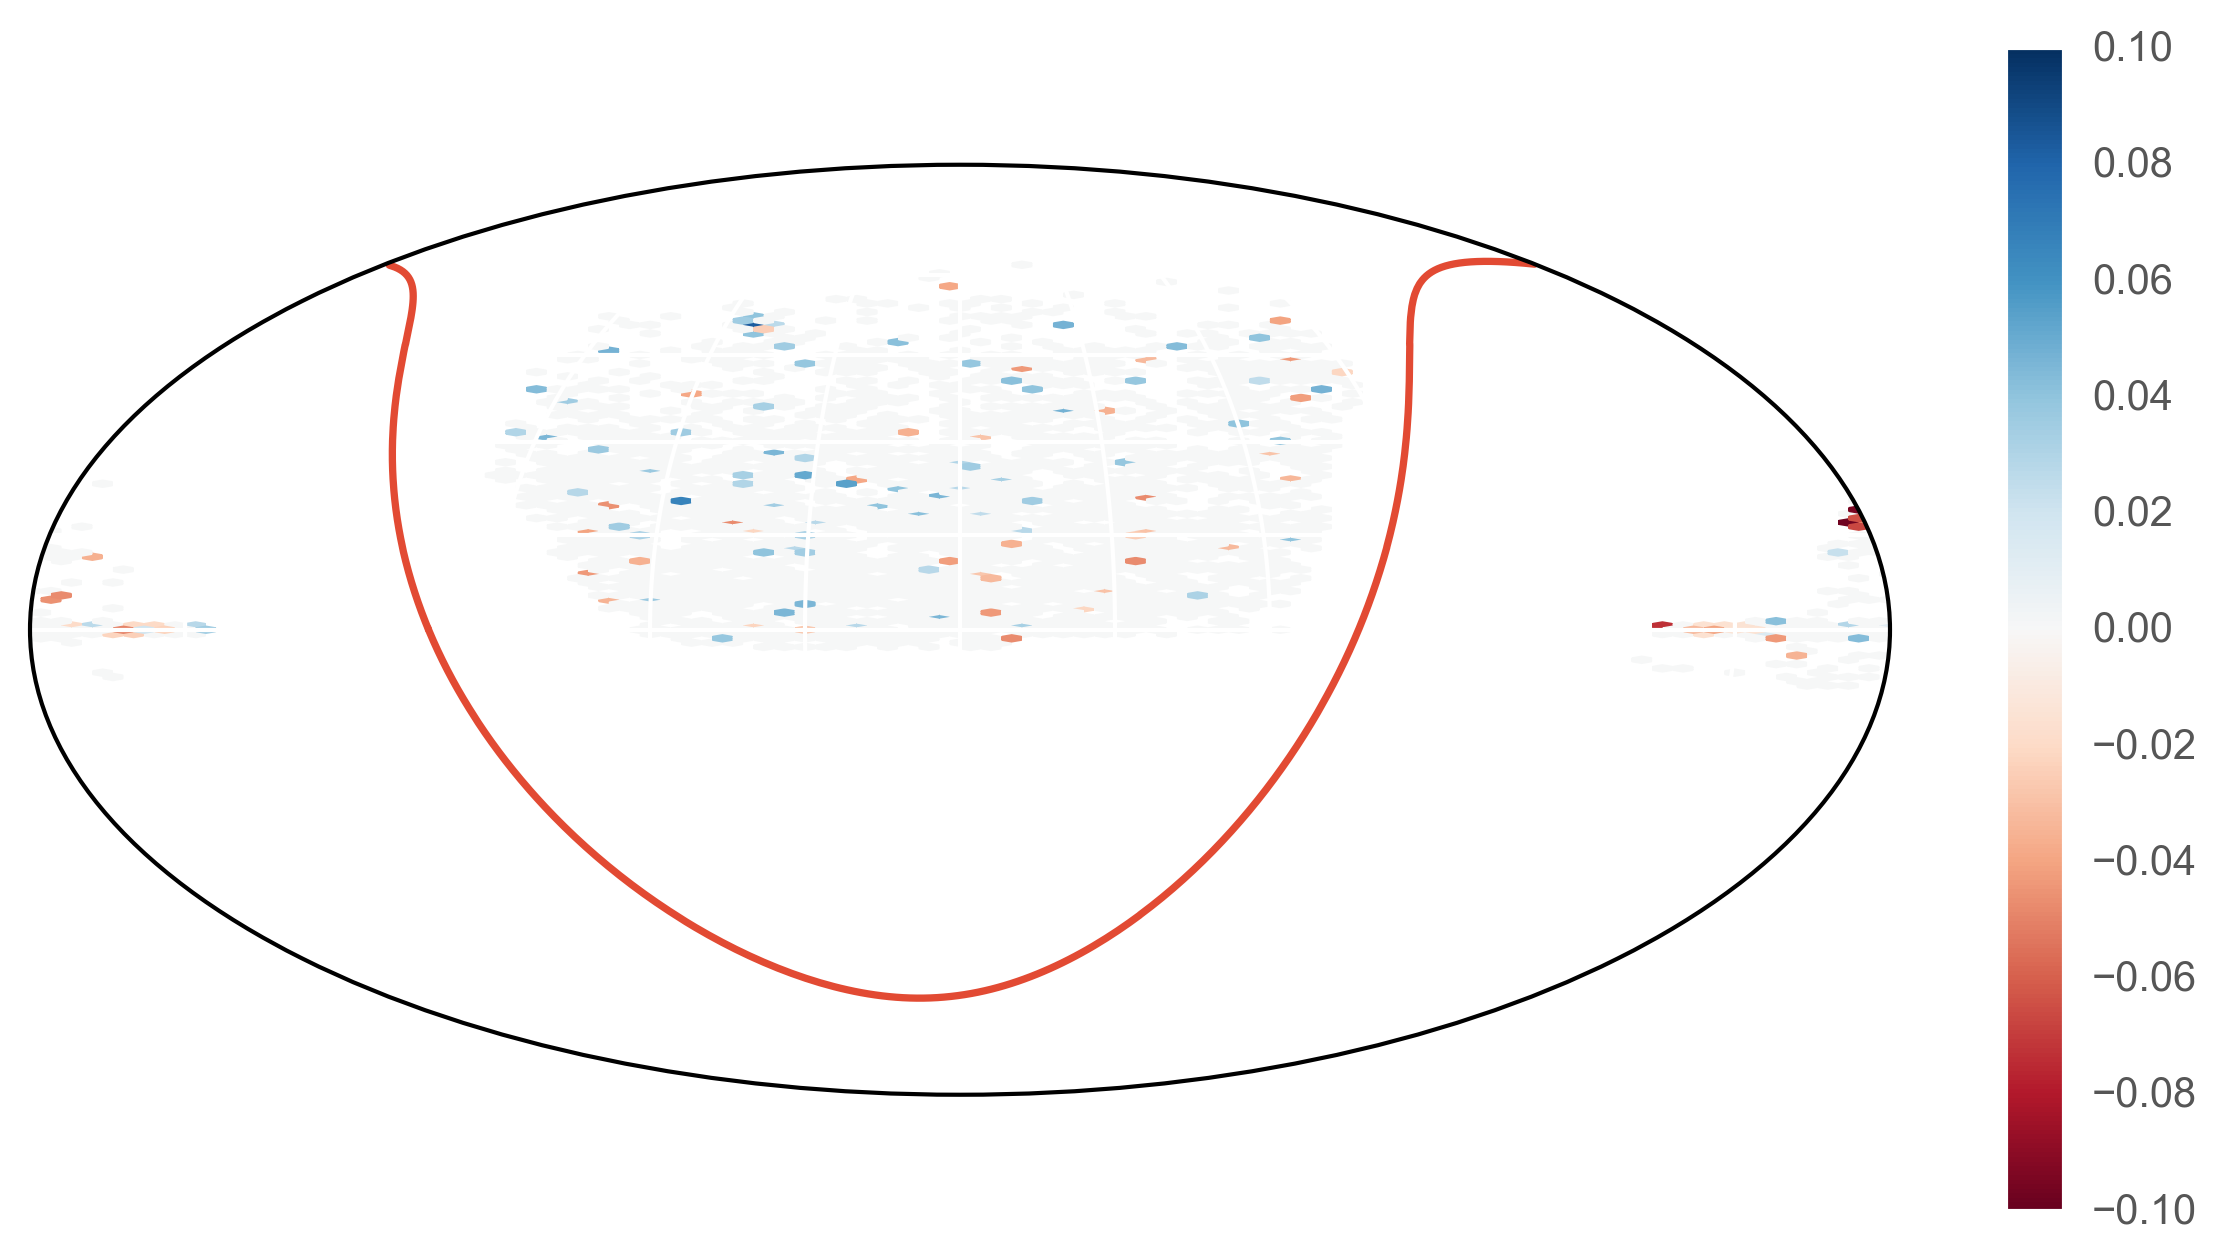
\includegraphics[width=0.75\textwidth]{figures/appendix/map_recall_sfd98_Galaxy}
		\caption{Recall improvement map of galaxies.}
		\label{fig:map_recall_sfd98_galaxies}
	\end{subfigure}\\
	\begin{subfigure}{\textwidth}
		\centering
		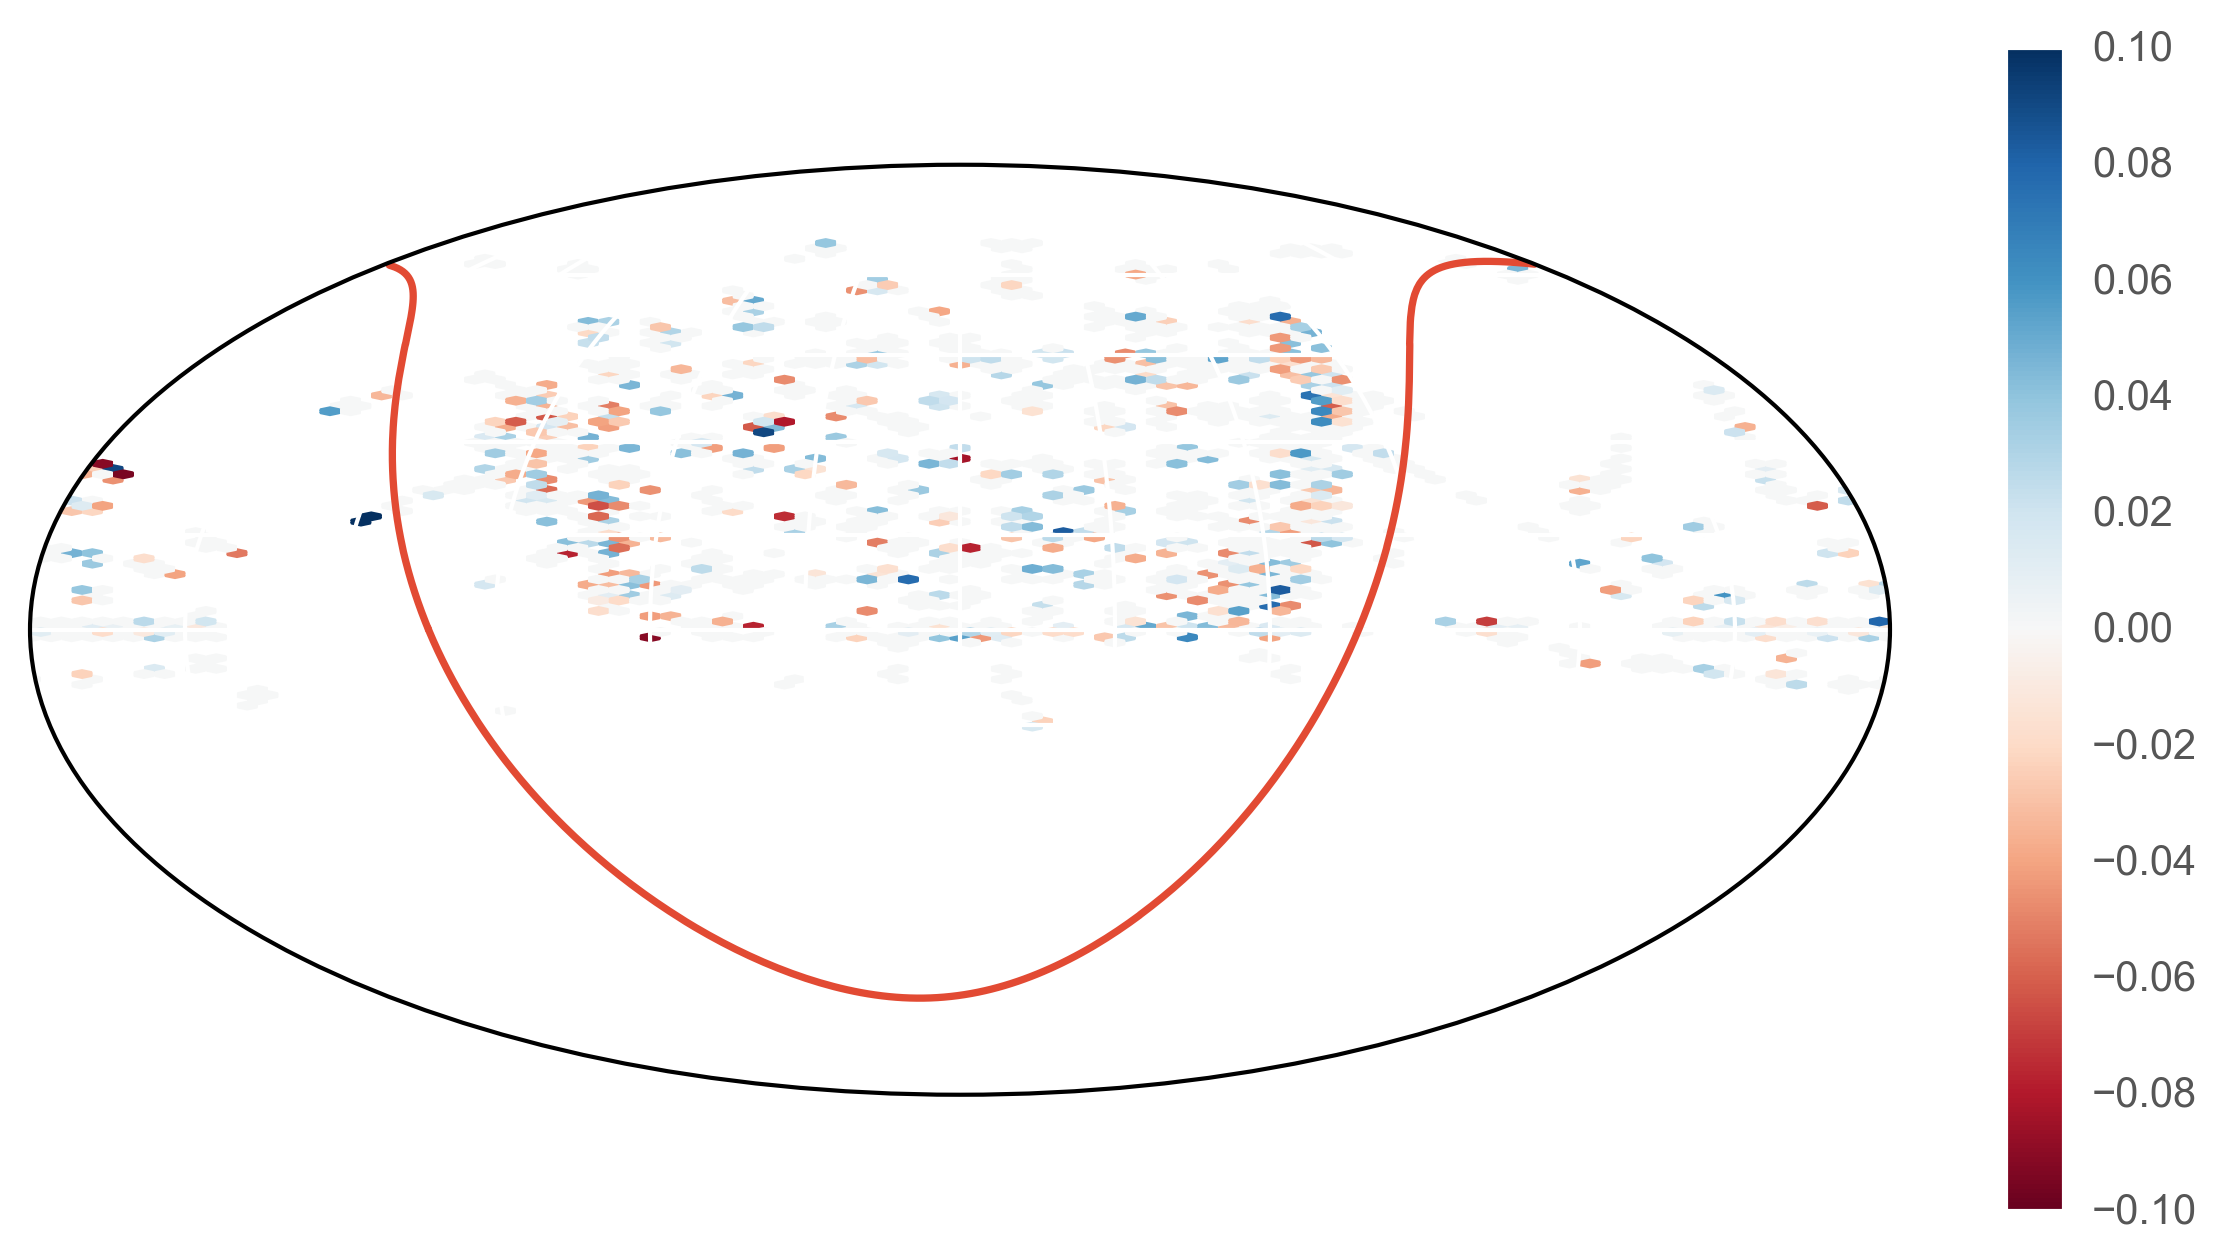
\includegraphics[width=0.75\linewidth]{figures/appendix/map_recall_sfd98_Star}
		\caption{Recall improvement map of stars.}
		\label{fig:map_recall_sfd98_stars}
	\end{subfigure}
	\begin{subfigure}{\textwidth}
		\centering
		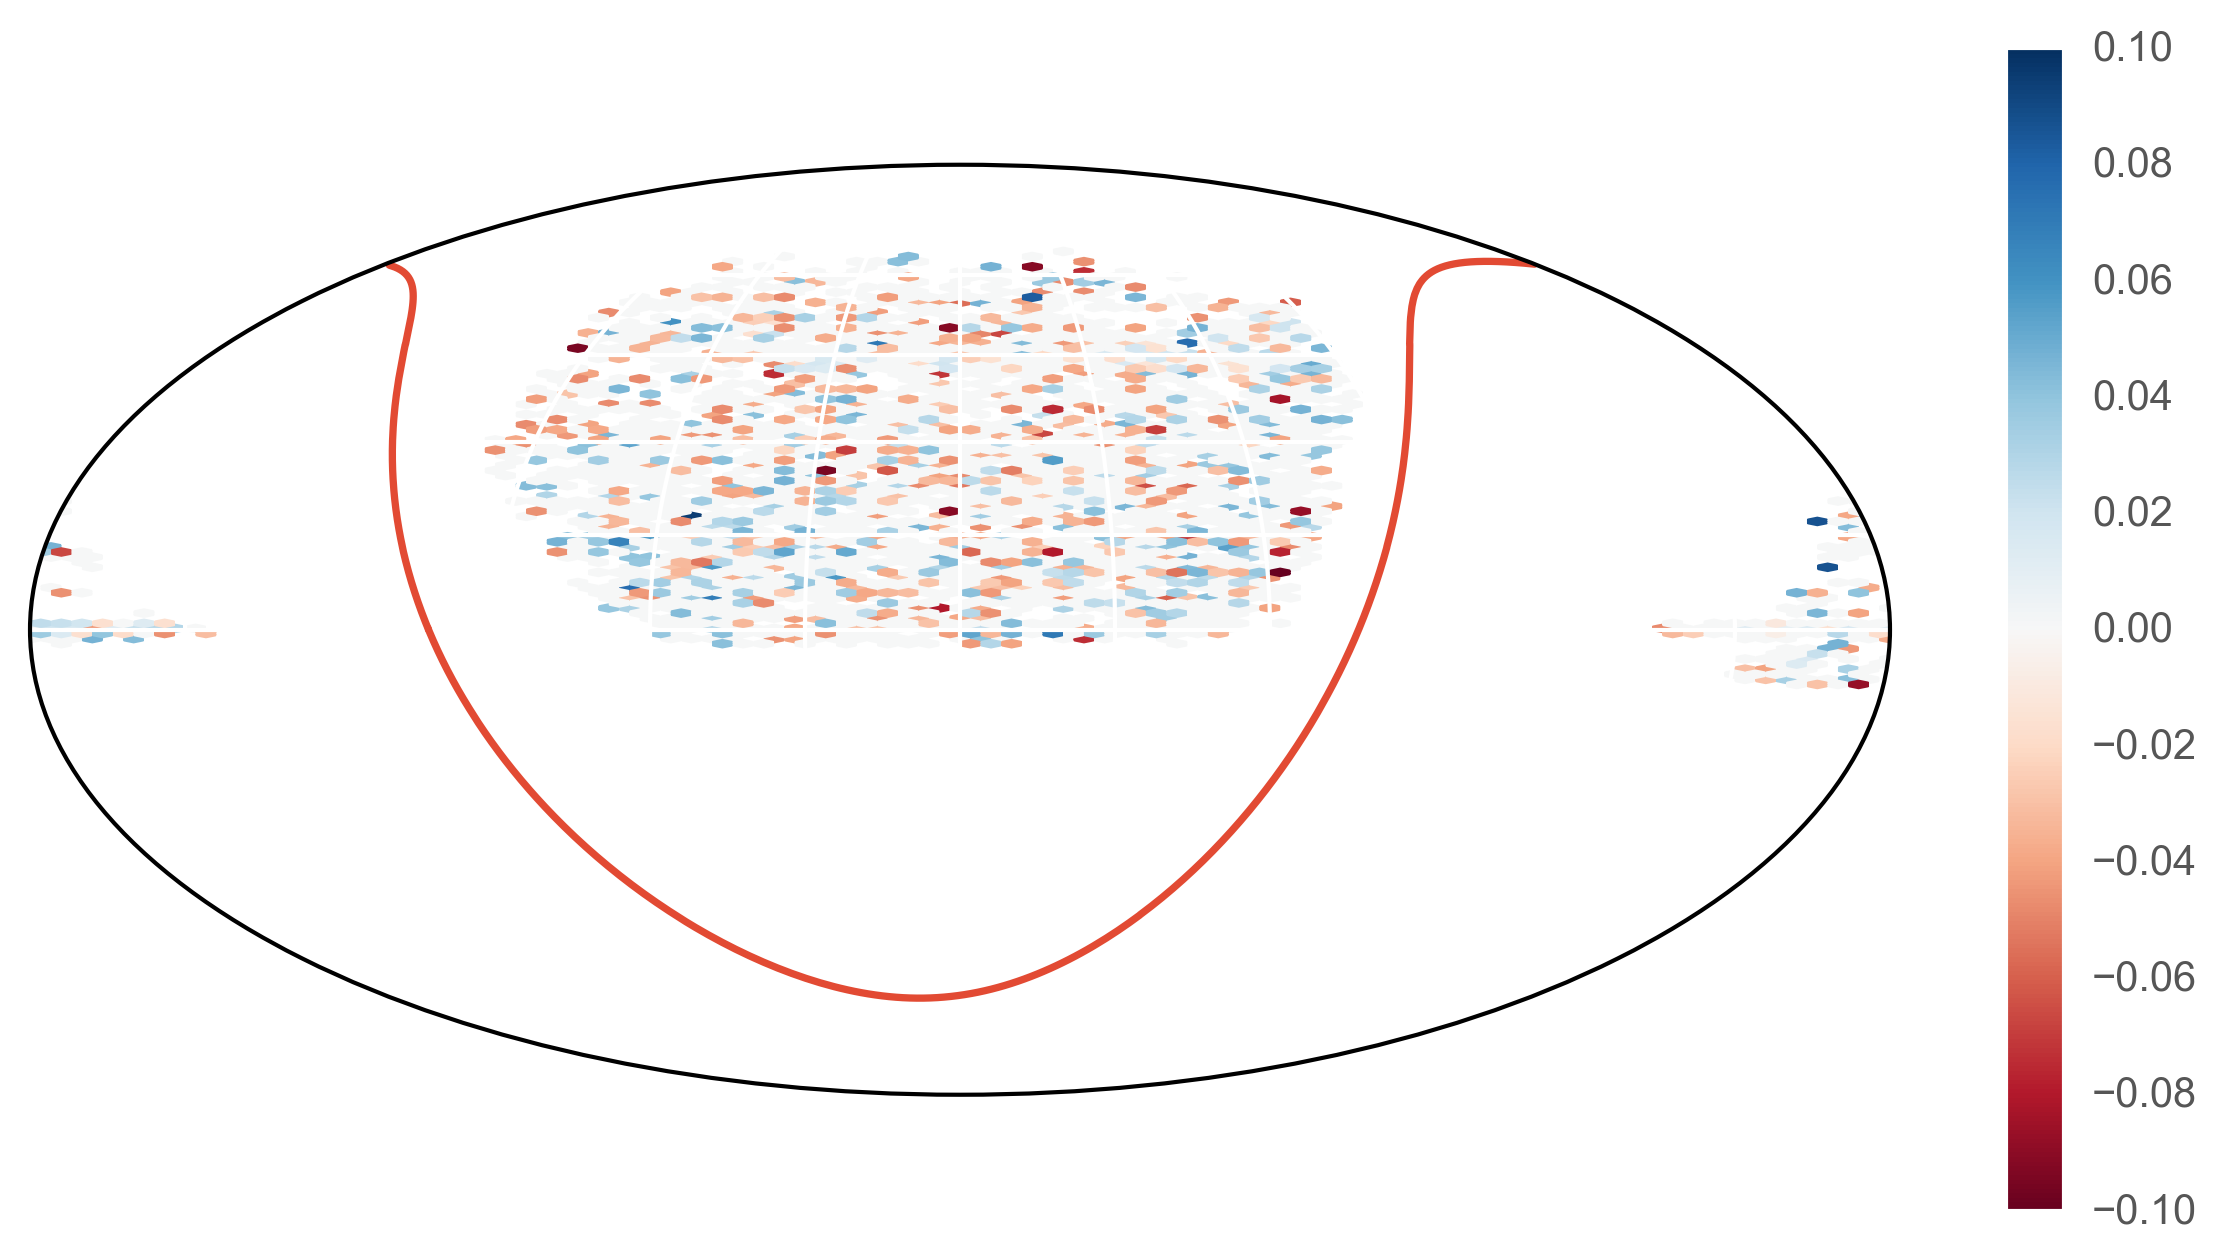
\includegraphics[width=0.75\linewidth]{figures/appendix/map_recall_sfd98_Quasar}
		\caption{Recall improvement map of quasars.}
		\label{fig:map_recall_sfd98_quasars}
	\end{subfigure}
	\caption[Recall improvement maps with SFD98]{
        Recall improvement maps when the SFD98 extinction vector is used.}
	\label{fig:map_recall_sfd98}
\end{figure}


\begin{figure}[p]
	\centering
	\begin{subfigure}{\textwidth}
		\centering
		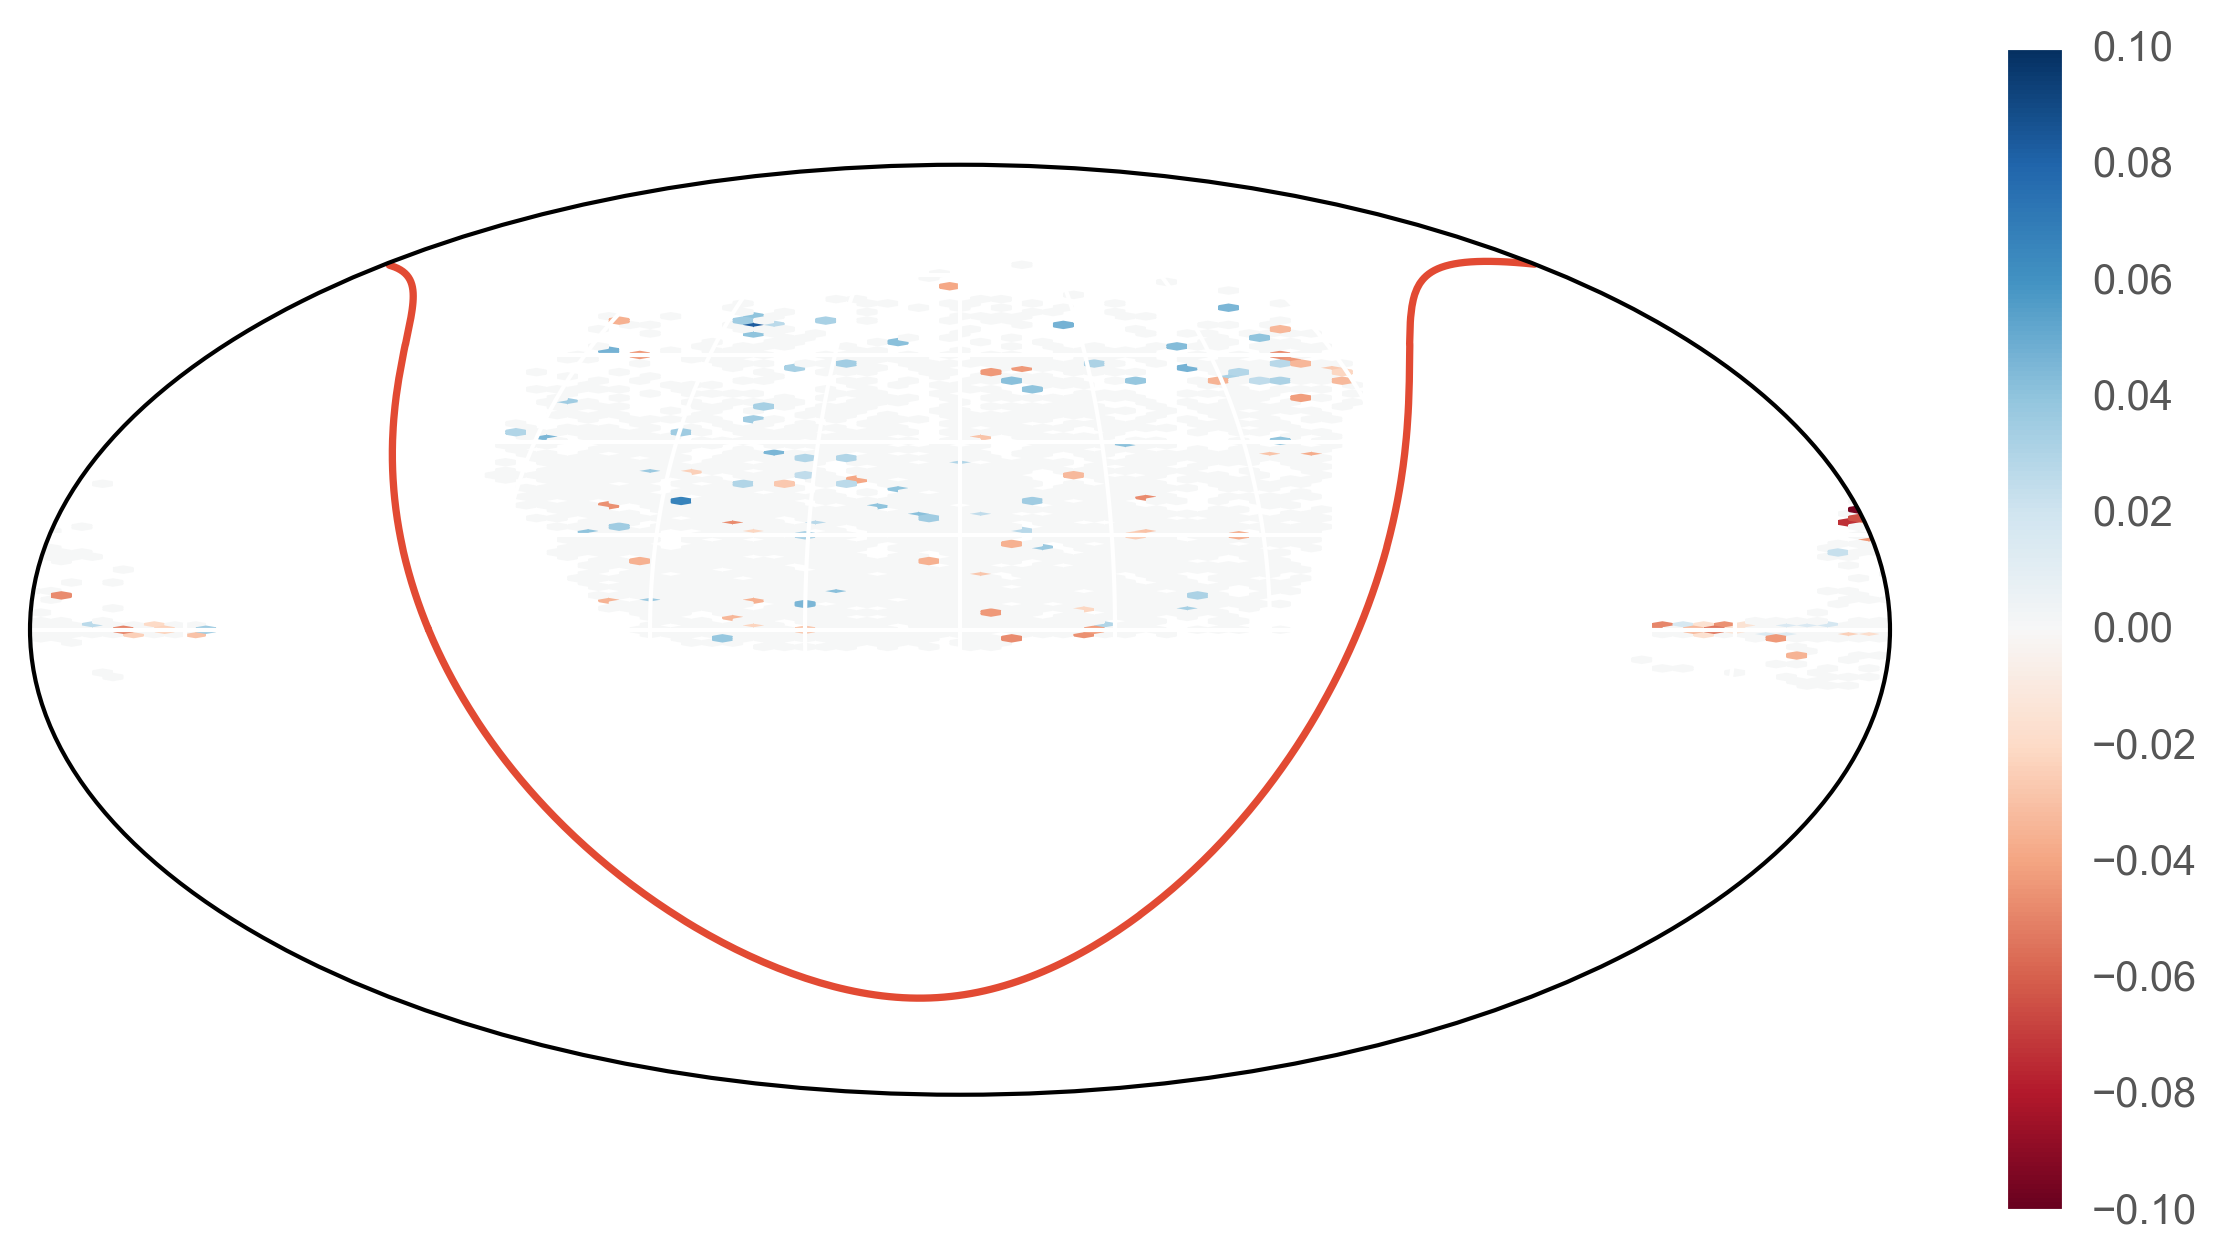
\includegraphics[width=0.75\textwidth]{figures/appendix/map_recall_sf11_Galaxy}
		\caption{Recall improvement map of galaxies.}
		\label{fig:map_recall_sf11_galaxies}
	\end{subfigure}\\
	\begin{subfigure}{\textwidth}
		\centering
		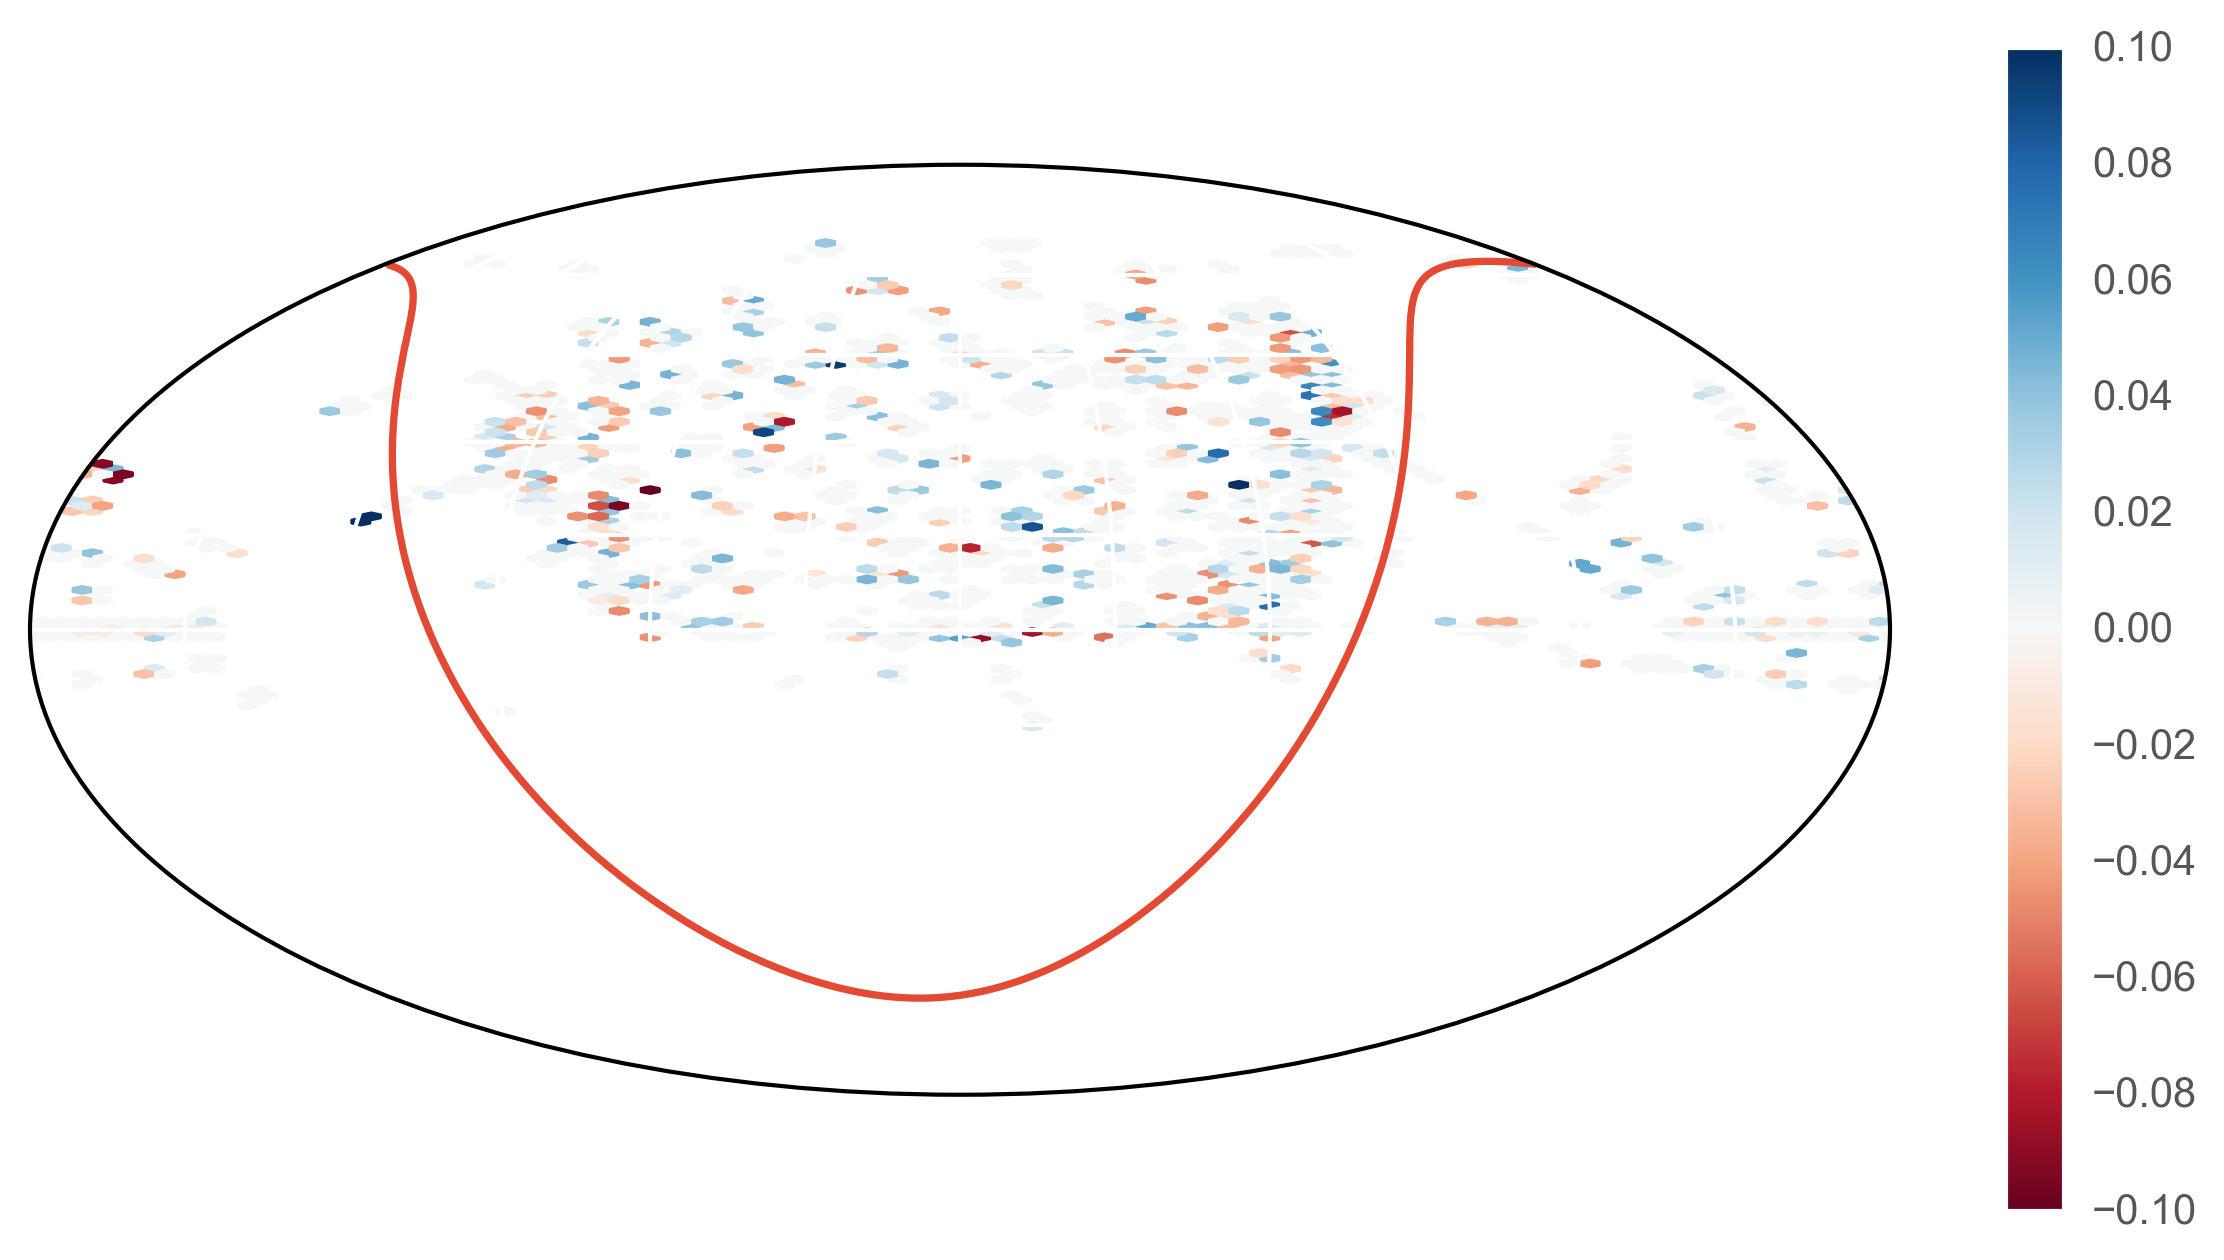
\includegraphics[width=0.75\linewidth]{figures/appendix/map_recall_sf11_Star}
		\caption{Recall improvement map of stars.}
		\label{fig:map_recall_sf11_stars}
	\end{subfigure}
	\begin{subfigure}{\textwidth}
		\centering
		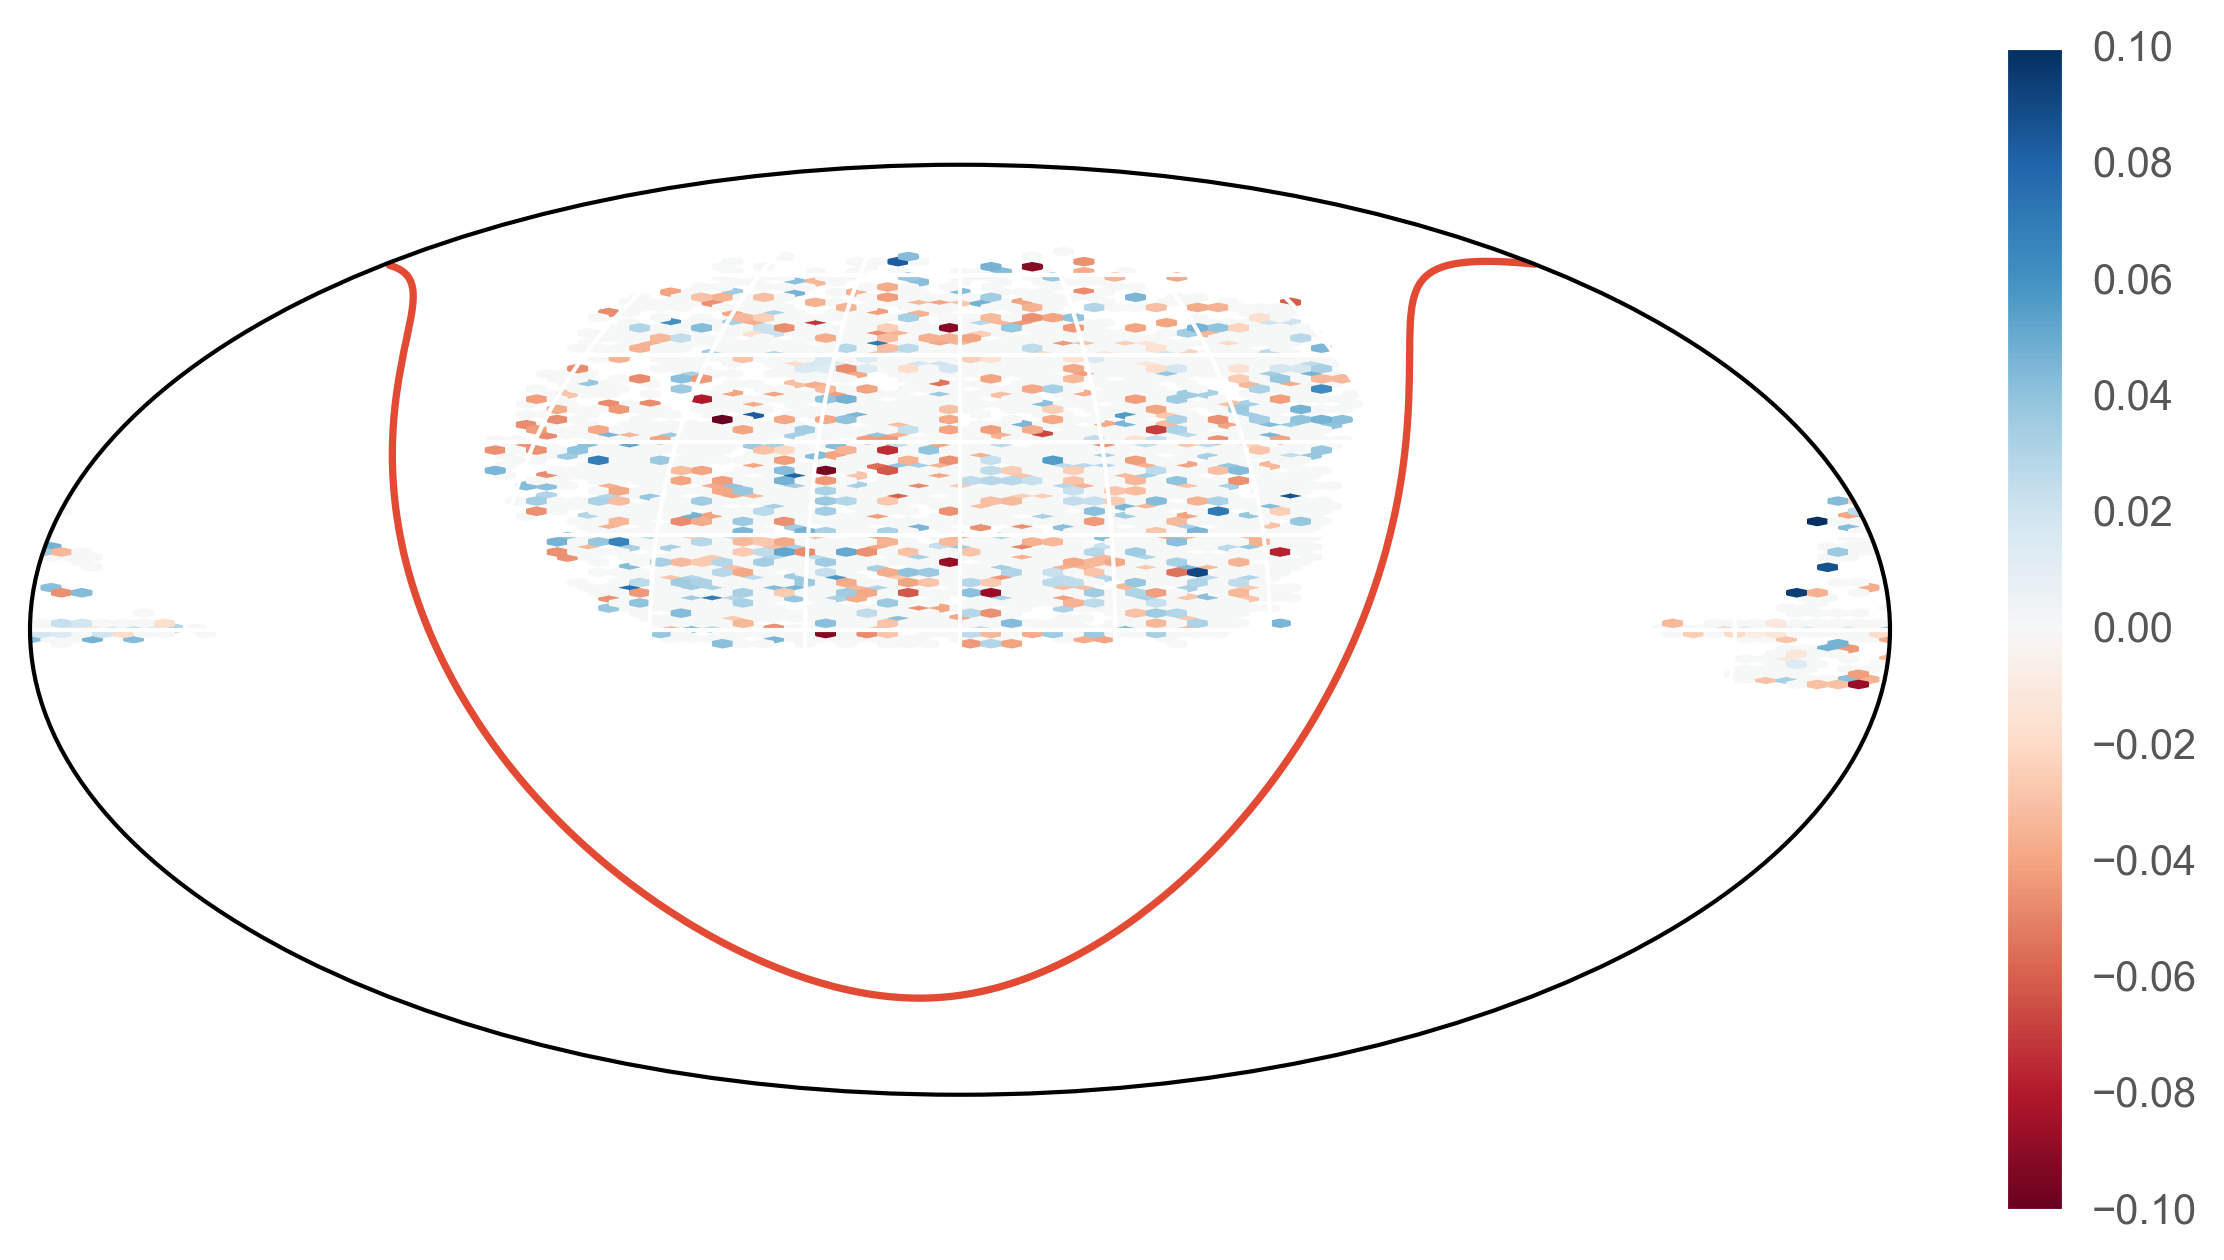
\includegraphics[width=0.75\linewidth]{figures/appendix/map_recall_sf11_Quasar}
		\caption{Recall improvement map of quasars.}
		\label{fig:map_recall_sf11_quasars}
	\end{subfigure}
	\caption[Recall improvement maps of when with SF11]{
        Recall improvement maps of when the SF11 extinction vector is used.}
	\label{fig:map_recall_sf11}
\end{figure}


\begin{figure}[p]
	\centering
	\begin{subfigure}{\textwidth}
		\centering
		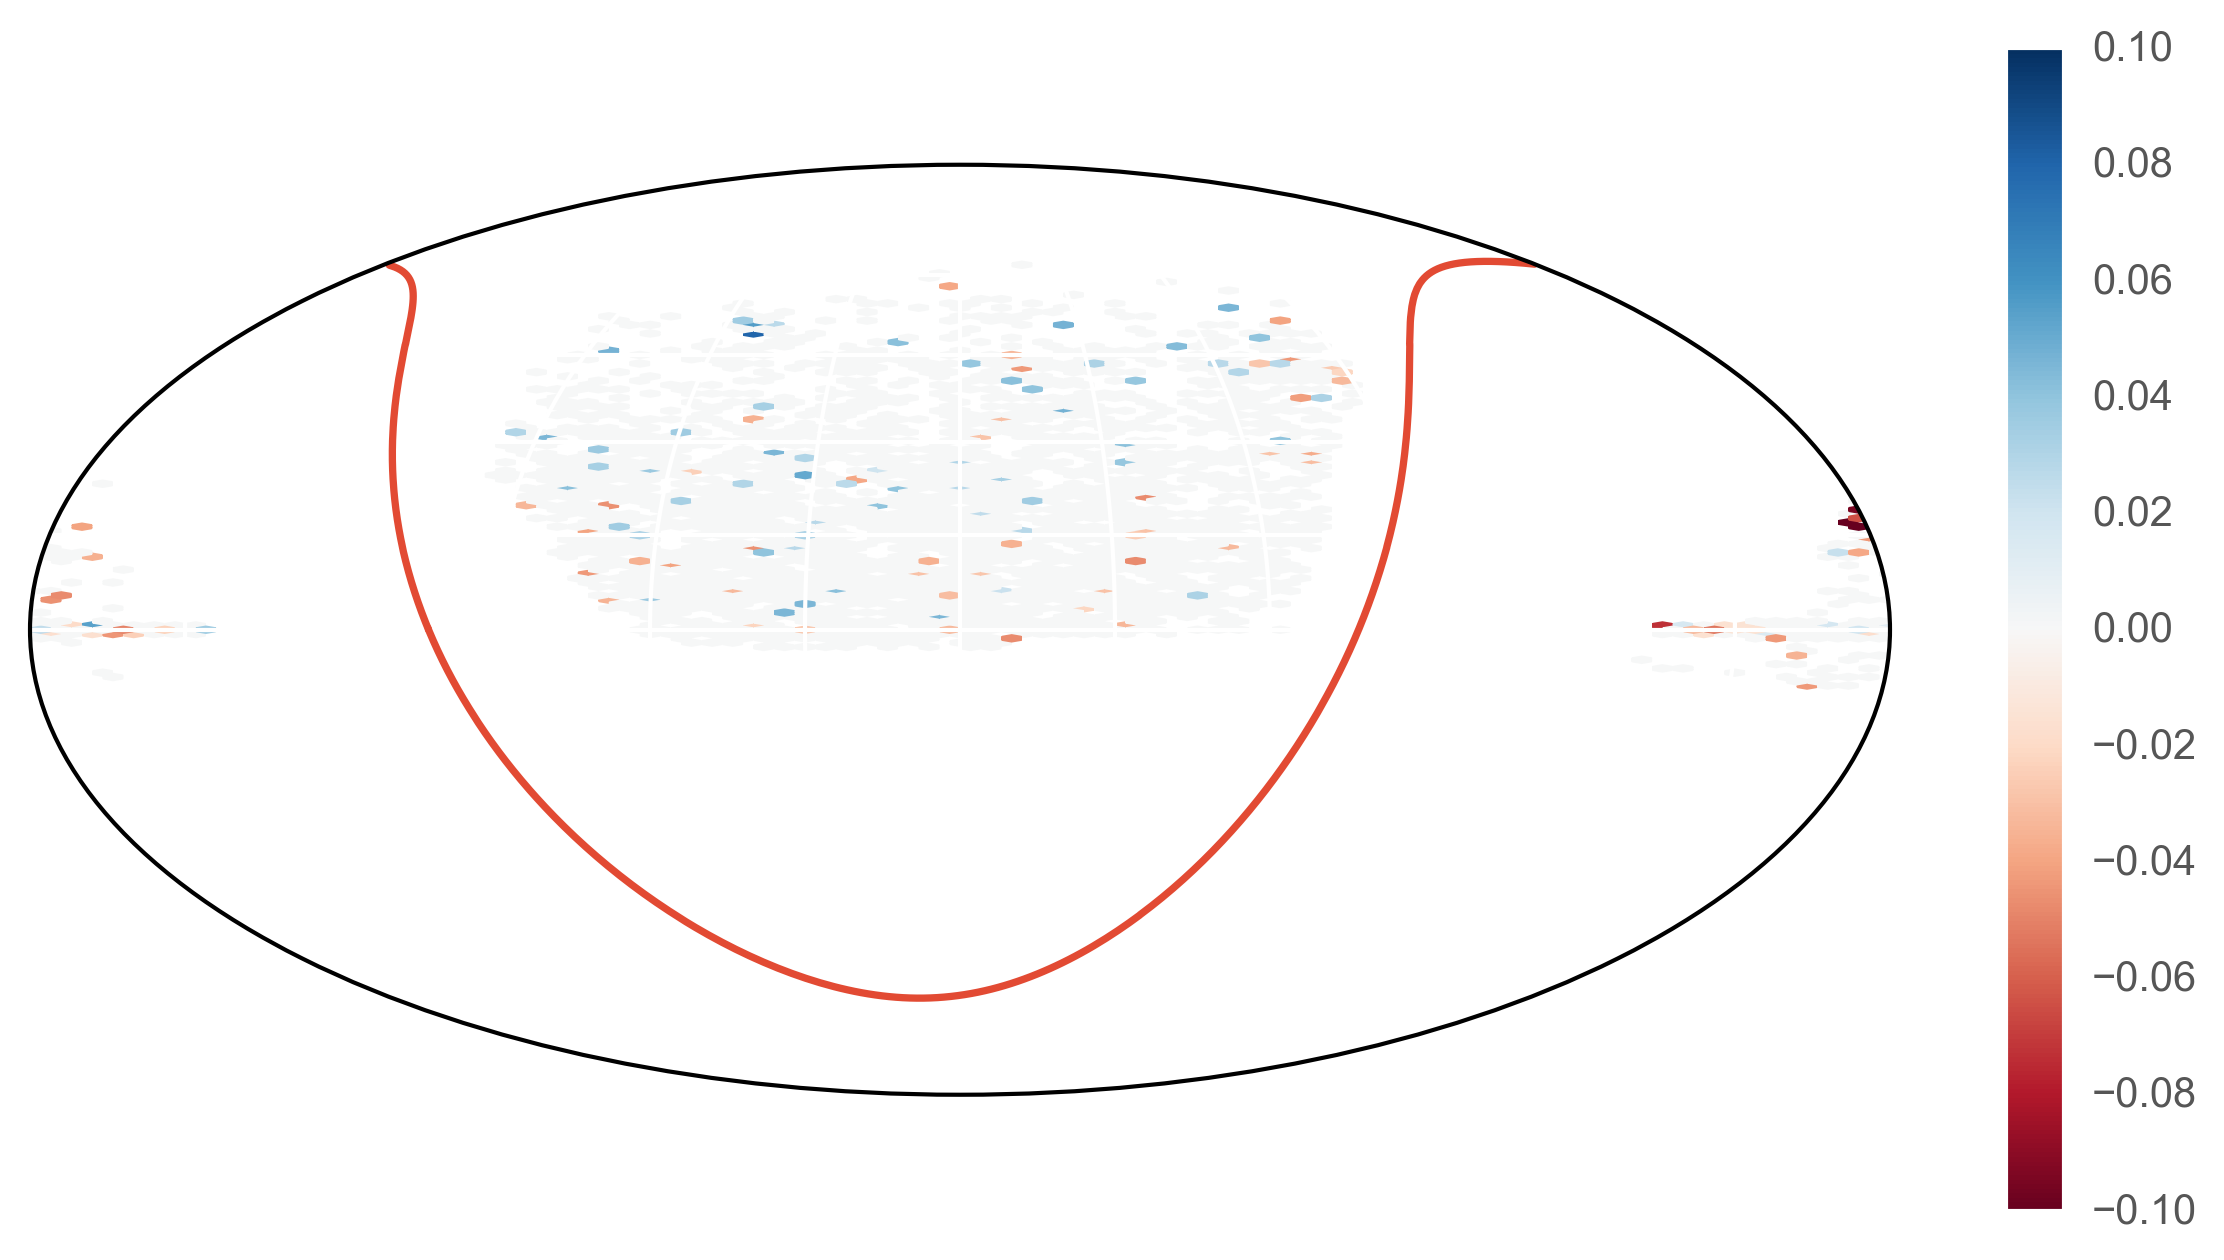
\includegraphics[width=0.75\textwidth]{figures/appendix/map_recall_w14_Galaxy}
		\caption{Recall improvement map of galaxies.}
		\label{fig:map_recall_w14_galaxies}
	\end{subfigure}\\
	\begin{subfigure}{\textwidth}
		\centering
		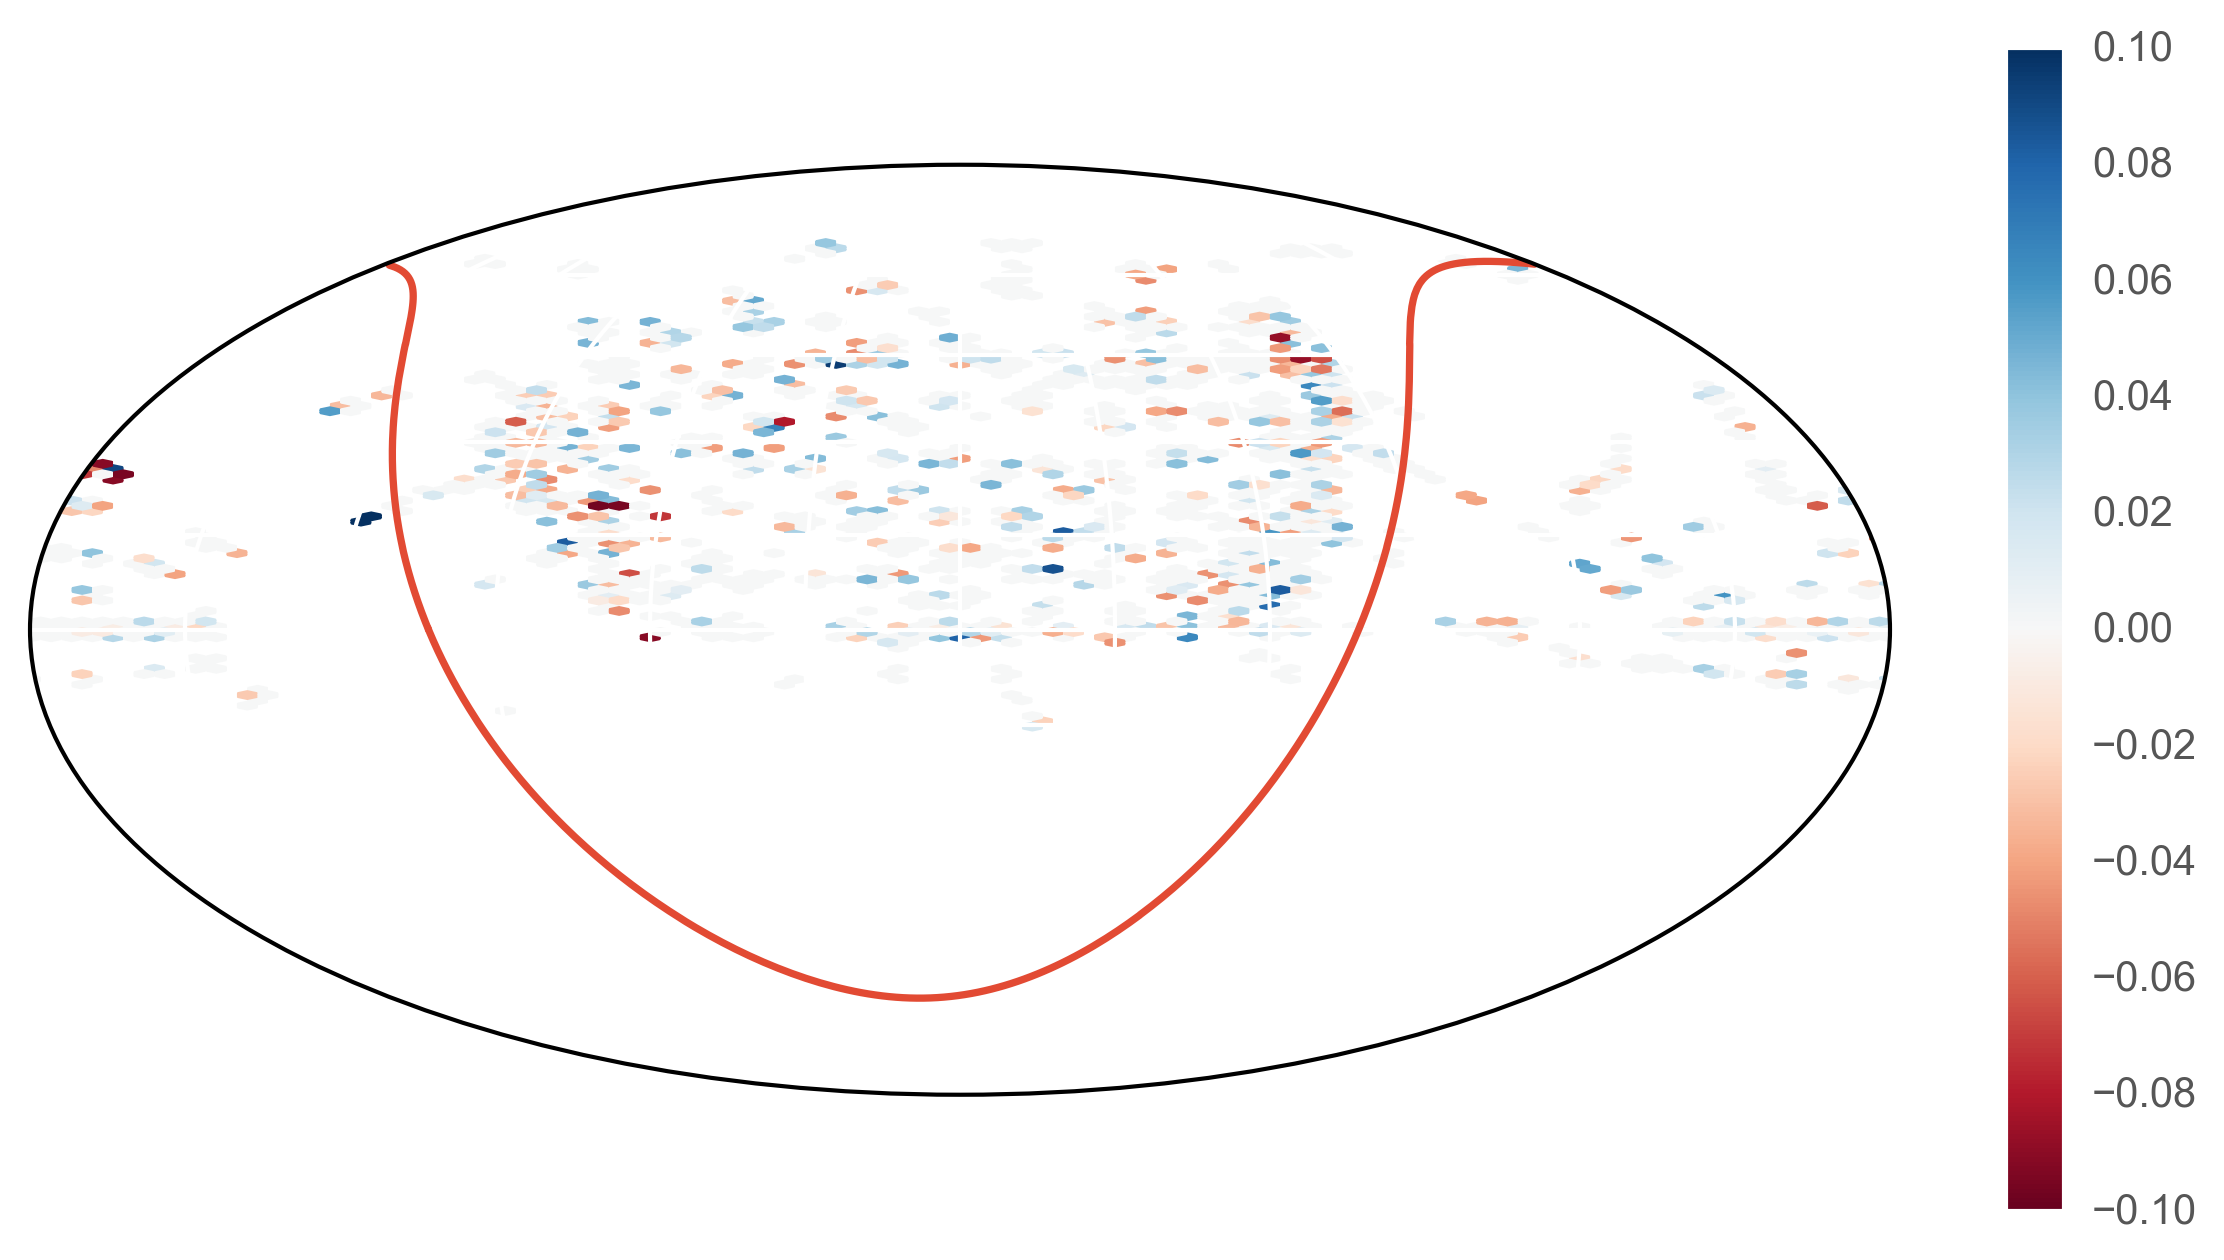
\includegraphics[width=0.75\linewidth]{figures/appendix/map_recall_w14_Star}
		\caption{Recall improvement map of stars.}
		\label{fig:map_recall_w14_stars}
	\end{subfigure}
	\begin{subfigure}{\textwidth}
		\centering
		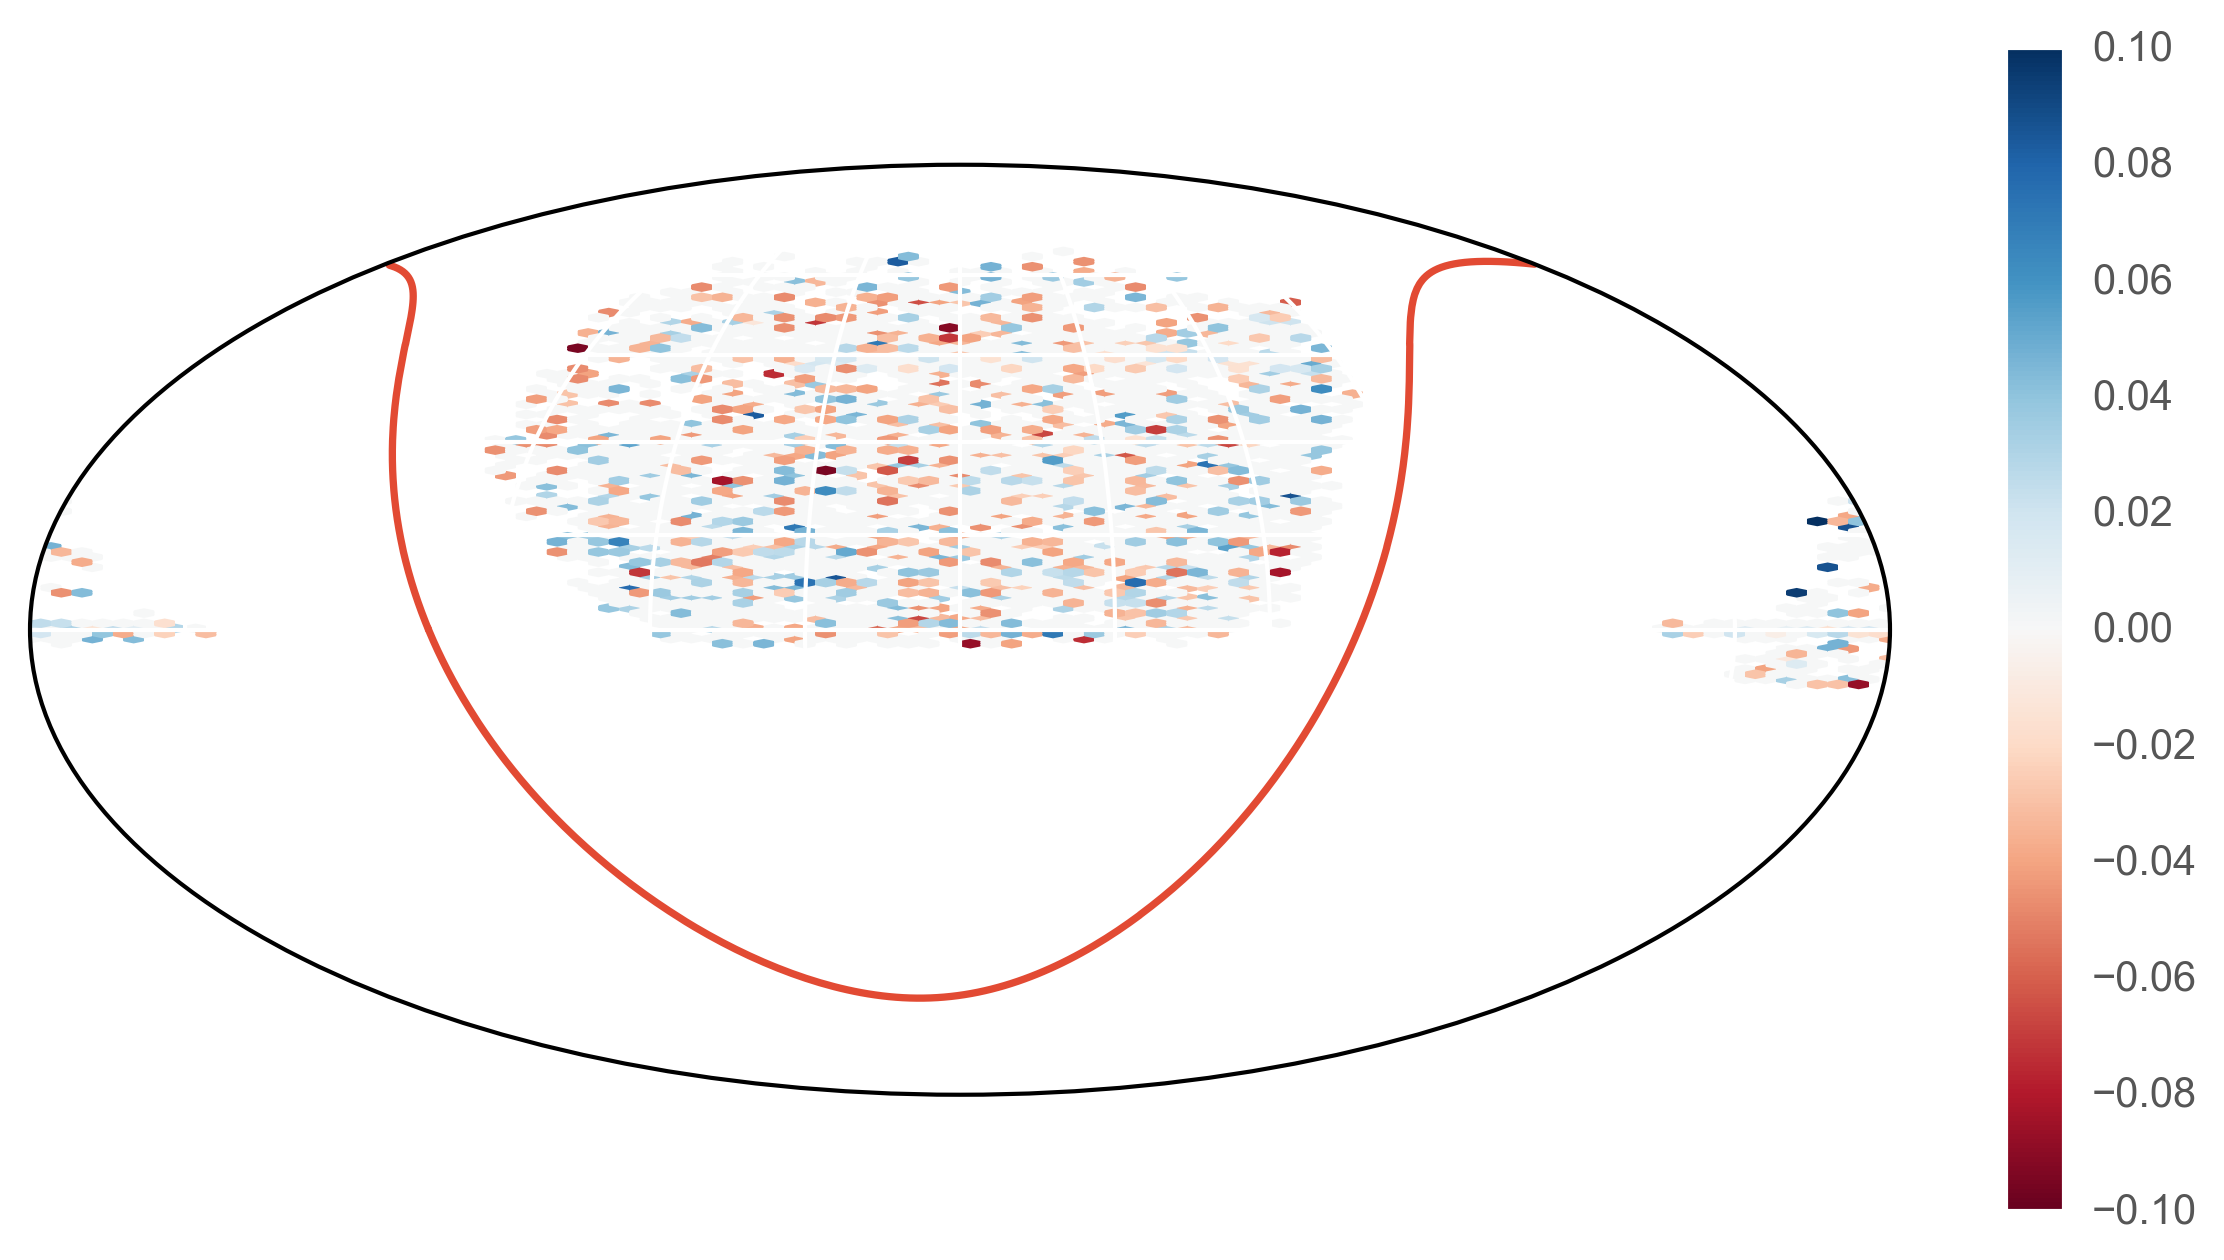
\includegraphics[width=0.75\linewidth]{figures/appendix/map_recall_w14_Quasar}
		\caption{Recall improvement map of quasars.}
		\label{fig:map_recall_w14_quasars}
	\end{subfigure}
	\caption[Recall improvement maps with W14]{
        Recall improvement maps of when the W14 extinction vector is used.}
	\label{fig:map_recall_w14}
\end{figure}



\section{Variance of the Mean Reward in Thompson Sampling}

Finally, Figures \ref{fig:sdss_sigmas} and \ref{fig:vstatlas_sigmas} show how $\sigma^2$,
the variance of the expected reward, changes with the training set size. As we would expect,
the variance decreases exponentially over time, since as we increase
the training size, we become more certain of the classifier's accuracy. In addition, the incremental change
of the accuracy rate shrinks over time as we approach an accuracy of 100\%.

\begin{figure}[p]
	\centering
	\begin{subfigure}{.5\textwidth}
		\centering
		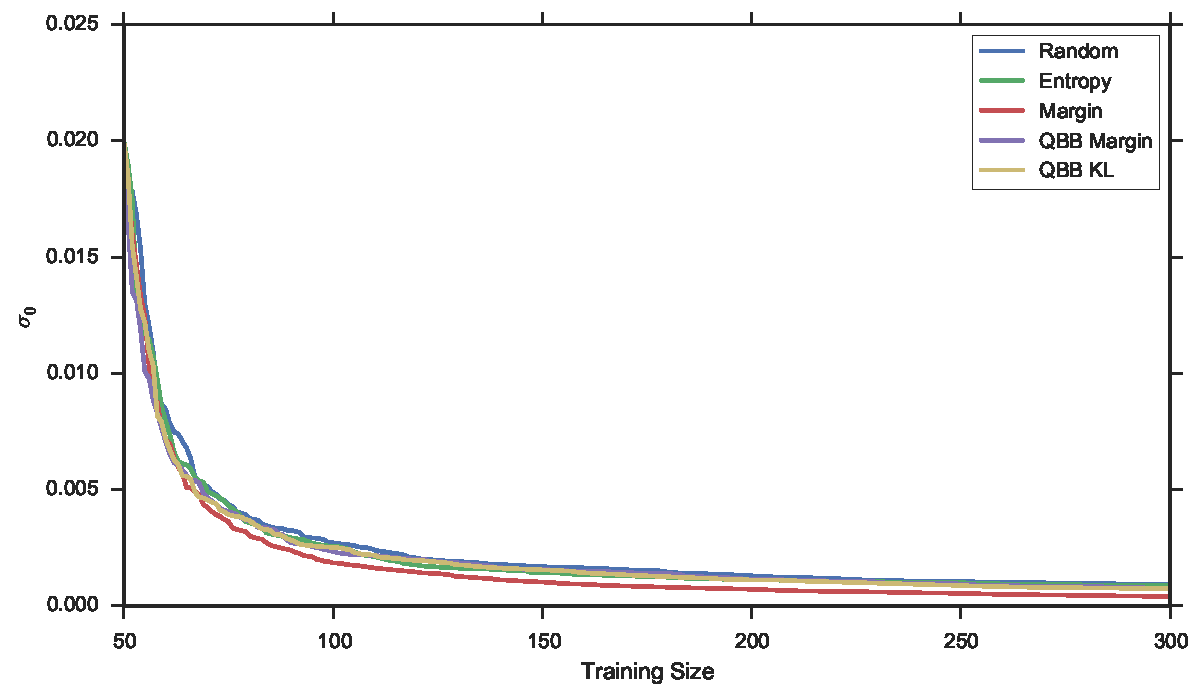
\includegraphics[width=\textwidth]{figures/5_thompson/vstatlas_bl_sigmas}
		\caption{Balanced pool and logistic regression}
		\label{fig:sdss_bl_sigmas}
	\end{subfigure}%
	\begin{subfigure}{.5\textwidth}
		\centering
		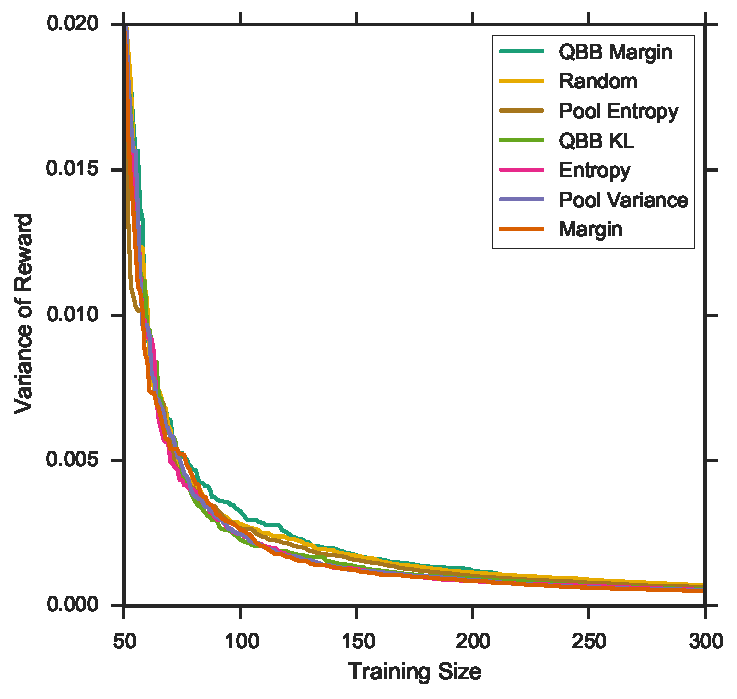
\includegraphics[width=\linewidth]{figures/5_thompson/sdss_br_sigmas}
		\caption{Balanced pool and RBF SVM}
		\label{fig:sdss_br_sigmas}
	\end{subfigure}
	\begin{subfigure}{.5\textwidth}
		\centering
		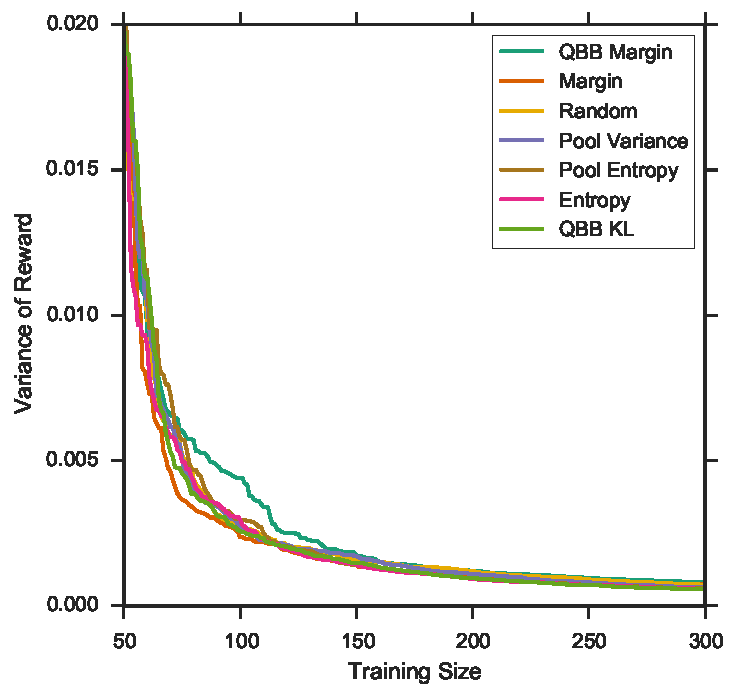
\includegraphics[width=\textwidth]{figures/5_thompson/sdss_ul_sigmas}
		\caption{Unbalanced pool and logistic regression}
		\label{fig:sdss_ul_sigmas}
	\end{subfigure}%
	\begin{subfigure}{.5\textwidth}
		\centering
		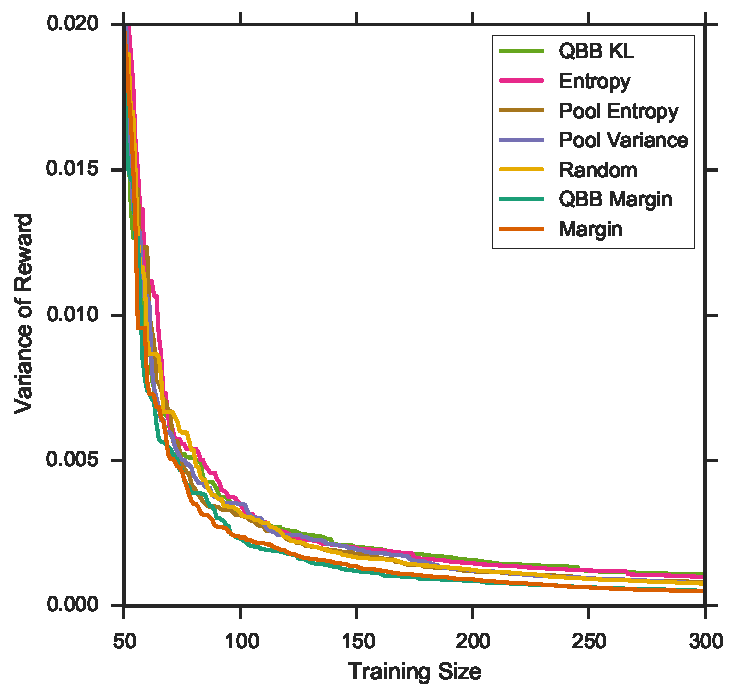
\includegraphics[width=\linewidth]{figures/5_thompson/sdss_ur_sigmas}
		\caption{Unbalanced pool and RBF SVM}
		\label{fig:sdss_ur_sigmas}
	\end{subfigure}
	\caption[Variance of the mean reward of heuristics (SDSS)]{
		Variance (average of 10 trials) of the expected reward in Thompson sampling with the SDSS dataset.}
	\label{fig:sdss_sigmas}
\end{figure}

\begin{figure}[p]
	\centering
	\begin{subfigure}{.5\textwidth}
		\centering
		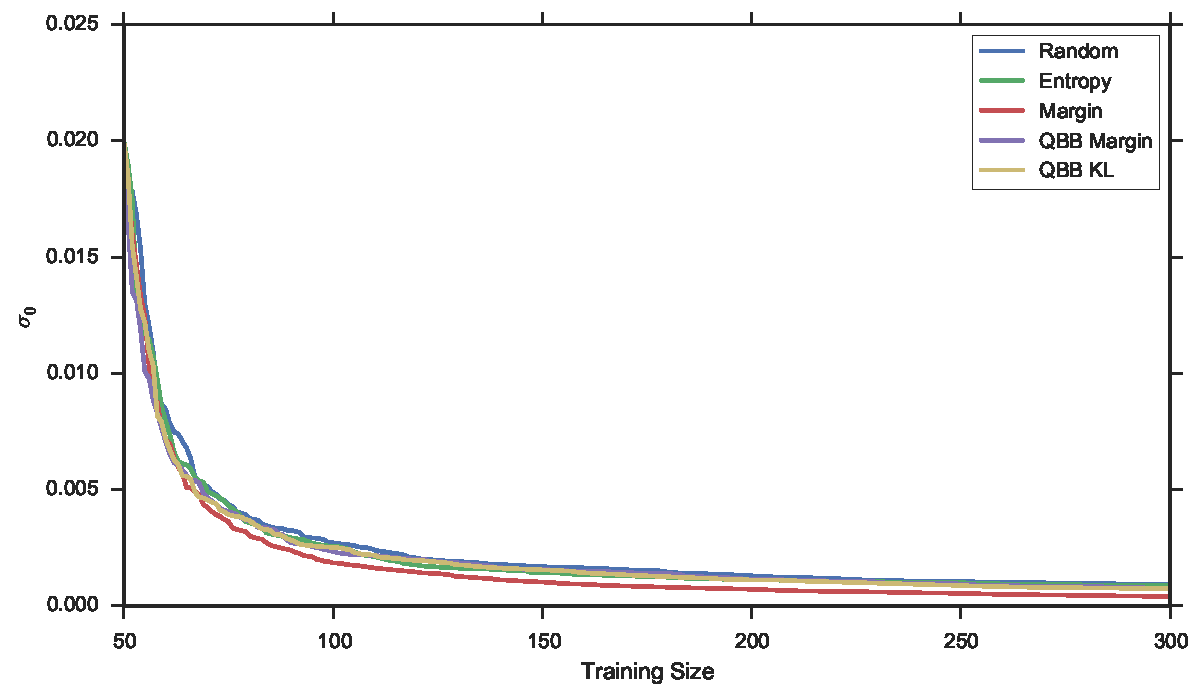
\includegraphics[width=\textwidth]{figures/5_thompson/vstatlas_bl_sigmas}
		\caption{Balanced pool and logistic regression}
		\label{fig:vstatlas_bl_sigmas}
	\end{subfigure}%
	\begin{subfigure}{.5\textwidth}
		\centering
		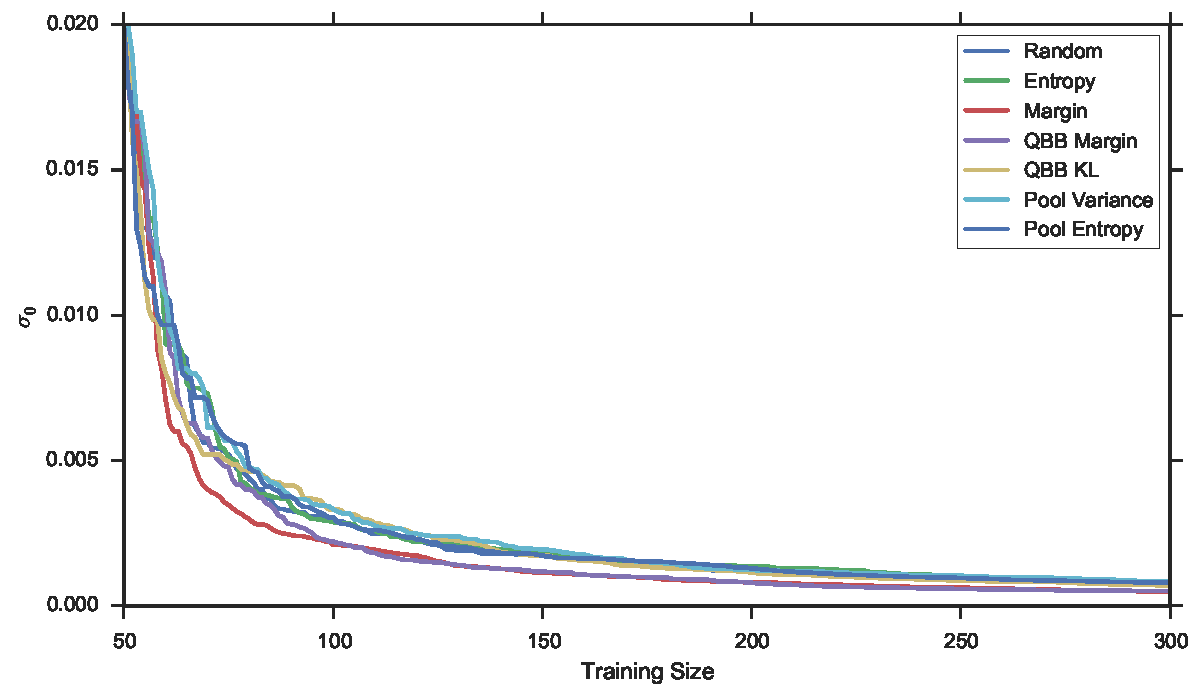
\includegraphics[width=\linewidth]{figures/5_thompson/vstatlas_br_sigmas}
		\caption{Balanced pool and RBF SVM}
		\label{fig:vstatlas_br_sigmas}
	\end{subfigure}
	\begin{subfigure}{.5\textwidth}
		\centering
		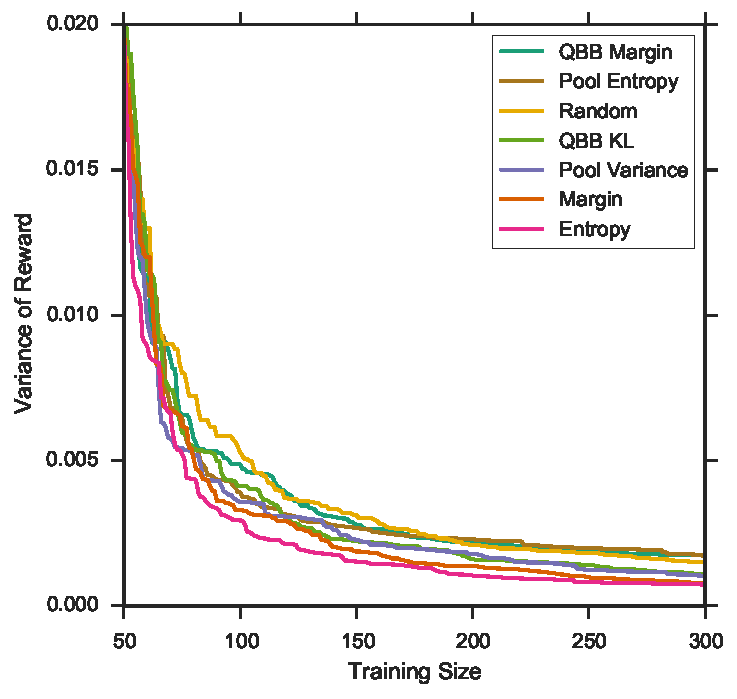
\includegraphics[width=\textwidth]{figures/5_thompson/vstatlas_ul_sigmas}
		\caption{Unbalanced pool and logistic regression}
		\label{fig:vstatlas_ul_sigmas}
	\end{subfigure}%
	\begin{subfigure}{.5\textwidth}
		\centering
		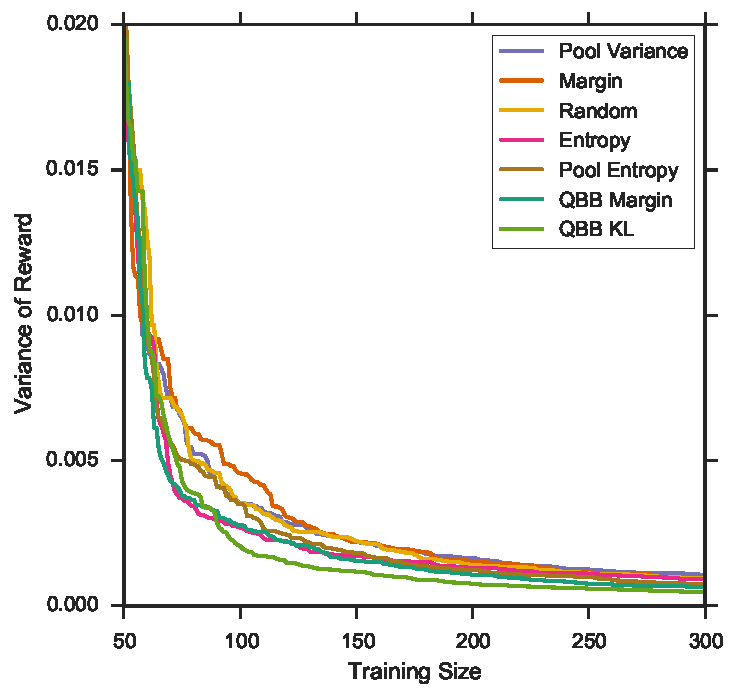
\includegraphics[width=\linewidth]{figures/5_thompson/vstatlas_ur_sigmas}
		\caption{Unbalanced pool and RBF SVM}
		\label{fig:vstatlas_ur_sigmas}
	\end{subfigure}
	\caption[Variance of the mean reward of heuristics (VST ATLAS)]{
		Variance (average of 10 trials) of the expected reward in Thompson sampling with the VST ATLAS dataset.}
	\label{fig:vstatlas_sigmas}
\end{figure}


%%% Local Variables: 
%%% mode: latex
%%% TeX-master: "thesis"
%%% End: 
